\chapter{\centering Implementation of CrazyOS}

\section{Introduction}
In the previous chapter we discussed our motivations behind creating a very basic operating system, CrazyOS. We described it as a single-user, single-tasking, real mode operating system. These three terms are described as follows:
\begin{enumerate}
  \item \textit{Single-user}: Most modern operating systems allow multiple user accounts. Each user has some disk space allocated to them and they can use it as they like. They can keep their personal files and projects separate from others work. Each user account is accessible through a password. CrazyOS does not support multiple users. It does not have the capability to communicate through a network with other computers. It is intended for one user only. No password logins are required to access the services of the system or to access the contents of a file.
  \item \textit{Single-tasking}: Modern operating systems allow users to run multiple programs at once. Each program is given its own address space to run without messing with other programs. Various scheduling algorithms, for example round-robin scheduling algorithm, are used to allocate a quantum of CPU's time to programs so that each program gets executed and give the user a feel of simultaneous execution of multiple programs. Threads and cores are also allocated to different batches of programs. CrazyOS is simple: it runs on a single processor and only a single program/process, which is the shell, is running most of the time. Other programs can be run either by passing commands from the shell, or by loading and running them from the disk.
  \item \textit{Real mode}: Modern operating systems run on 64-bit CPUs. One such CPU is the x86-64 family of processors produced by both AMD and Intel. These processors use 64-bit registers and address space and use paging (i.e., creation of virtual address spaces) to protect programs from each other. To provide backwards compatibility to programs which would run only on 32-bit and 16-bit machines, x86-64 processors initially run as 16-bit processors when the machine has just been powered on. In this mode, they try to act like an 8086 processor. This mode of operation is called \textit{real mode} or \textit{virtual 8086 mode}. After going through a complex setup procedure, the user can use the processor in 32-bit mode which is called \textit{protected mode}. After some more setting up, the user can finally run the processor in 64-bit or \textit{long mode}. In this mode, programs can utilize all the capabilities of the processor. Most modern operating systems run in long mode. However, to reduce complexity of its design and to make it relevant for use as a tool in courses on computer architecture and 8086 microprocessor, CrazyOS runs in real mode or virtual 8086 mode only.   
\end{enumerate}
The implementation of CrazyOS is presented in this chapter. We will begin by describing the build environment and organization of the source files. Integral components of the operating system are then discussed in detail.

\section{Set-up of the Development Environment}
The development environment of CrazyOS consists of five software tools: code editor, assembler, emulator, build automation software, and source version control software. We will now explain the tools of choice for this project.

\subsection{Code Editor}
Earlier versions of the operating system were written using gVim. As the size of the project grew, the author found it difficult to maintain files using gVim. Therefore, a switch to VScode was made and it has since become the default code editor for this project. \textit{x86 and x86\_64 Assembly} syntax highlighting extension was downloaded as it supported NASM's syntax. Github's dark theme is used as the author find it to be pleasing to his eyes.

\subsection{Assembler}
Many assemblers supporting the x86 architecture are available. The author had the choice of using either GNU AS or NASM. GNU AS is a part of GCC and supports multiple architectures. Due to this reason, it is used for developing and maintaining assembly source files in many projects such as the Linux kernel. However, it by default uses AT\&T syntax which is different from Intel syntax, the latter being found in datasheets and software developer's manuals provided by both AMD and Intel. Few of the differences between AT\&T and Intel syntax are listed below:
\begin{enumerate}
  \item Intel syntax requires that after writing the instruction, the user has to first mention the destination operand and then the source operand. AT\&T syntax requires that the source operand is to be mentioned first. Therefore, \texttt{mov eax, ebx}, written in Intel syntax, and \texttt{movl \%ebx, \%eax}, written in AT\&T syntax, are both equivalent to each other.
  \item Register names are prefixed with \verb|%|, immediate and static operands with \verb|$| and hexadecimal numbers are prefixed with \texttt{0x}.
  \item Size of the operands is to be mentioned by suffixing a literal(s) with the instruction mnemonic. Three most commonly used literals are \verb|b| for byte operands, \verb|w| for word operands, and \verb|l| for doubleword operands.  
\end{enumerate}
Therefore, \texttt{mov byte [bx], al}, written in Intel syntax, and \texttt{movb \%al, (\%bx)}, written in AT\&T syntax, are equivalent to each other. Being a beginner himself, the author found out that it takes sometime to get used to AT\&T syntax. Furthermore, GNU AS partially supports Intel syntax and its documentation was found to be bit terse at places. Therefore, the author decided to use the Netwide Assembler, or NASM as it is usually called, for assembling the source files. NASM supports only x86 and x86-64 architecture and by default uses Intel syntax. It has a rich set of preprocessor directives which make it easier to include files and write macros. It can output assembled files in many different formats, such as ELF, plain binary, COM, etc. An excellent documentation is also provided by the NASM development team \cite{nasm2015doc}.

\subsection{Emulator}
The author had a bad experience with emu8086 which is widely used in courses dealing with 8086 microprocessor in Indian colleges. The emulator comes with a free trial period of 14 days after which a license needs to be purchased. The emulator's free trial ended on the day of practical examination, which infuriated all of his colleagues including the author himself. He also found it to be impossible to link his own software with the emulator, which the documentation stated was possible.\\
During the development of CrazyOS, the author had the choice to either use VMware Workstation Player or QEMU. Both of these software are used by professionals for testing operating systems, with the former being a virtualization software and the latter being an emulator. A virtualization software allows the user to run a guest OS meant for the same architecture on which the host OS is running. Resources of the system are managed by the virtualization software, in this case VMware Workstation Player. In the case of an emulator, software fills in the role of hardware by emulating hardware devices. An emulator allows the user to run software which is meant for different architectures. QEMU uses kernel-based virtual machine which uses translation of guest machine's instructions to host machines at byte level, which allows it to run guest OS at near native speed \cite{bellard2005qemu}.\\
VMware Workstation Player was found to be using too many resources when running Windows XP on the author's laptop. It was also found that it was not able to boot CrazyOS properly. As the author found QEMU to be able to run Windows XP and toy operating systems with ease on his machine, he chose it over VMware Workstation Player and has used it for testing CrazyOS. In particular, QEMU's emulation of an IBM PC using i386 (80386) microprocessor has been used for testing the operating system. This emulator is ran from the terminal using the command \verb|qemu-system-i386|. Emulation of various peripherals and disk drives can be connected to it using by specifying them with typing appropriate commands after typing the name of machine to be emulated. For example, if the user has a binary file, \verb|file.bin| which he wishes to use a floppy disk A for an i386 based IBM PC, he can do so by executing the following command:\\
\texttt{qemu-system-i386 -fda file.bin}

\subsection{Makefile}
GNU Make is widely used by developers across the globe for building object files and executables automatically without retyping commands for building each source file. The author has used a single makefile, \verb|CrazyOS/8086/Makefile|, for building the image of the operating system.

\subsection{Git}
Git is the most popular source version control software. It used for maintaining many big open source projects such as the Linux kernel and VScode. A local Git repository can be linked to a remote repository on the internet. Most developers use Github as the platform for hosting their projects and collaboratively developing and maintaining them. The author has used Git v2.34.1 for maintaining this project. The project is hosted at \url{https://github.com/PraneetKapoor2619/CrazyOS}, with the latest short commit ID as of writing this report being \href{https://github.com/PraneetKapoor2619/CrazyOS/tree/1a17fa09b6df15038edabdefe9fd9ab04cb80907}{1a17fa0}.   

\section{Structure of the Project Directory}
CrazyOS started out as a project to teach its author about the 8086 microprocessor and the IBM PC. The author expects to write similar toy operating systems for computers using i386, x86-64, ARM and RISC-V processors. These ambitions are reflected in the commit history and by the structure of the project directory. We will begin by explaining the structure of the parent directory, \verb|CrazyOS/|. The rest of this chapter and the report will be concerned with the contents of \verb|CrazyOS/8086/| directory.

\subsection{Parent Directory}
Assuming the reader clones the project from Github into a directory named \verb|CrazyOS|, the directory tree that will be obtained is shown in \autoref{fig:parentdirtree}. \textit{depth = 0} indicates the number of files and subfolders that are being shown in the source tree.\\

\begin{figure}[H]
\begin{forest}
  for tree={
    font=\ttfamily,
    grow'=0,
    child anchor=west,
    parent anchor=south,
    anchor=west,
    calign=first,
    edge path={
      \noexpand\path [draw, \forestoption{edge}]
      (!u.south west) +(7.5pt,0) |- node[fill,inner sep=1.25pt] {} (.child anchor)\forestoption{edge label};
    },
    before typesetting nodes={
      if n=1
        {insert before={[,phantom]}}
        {}
    },
    fit=band,
    before computing xy={l=15pt},
  }
[CrazyOS
  [8086]
  [cos]
  [Documentation]
  [.git]
  [LICENSE]
  [README.md]
  [.gitignore]
]
\end{forest}
\caption{Parent directory tree (depth = 0)}
\label{fig:parentdirtree}
\end{figure}

The reader will observe that there is a folder named \verb|8086|. It contains the source files for building 16-bit real mode version of CrazyOS which is the subject matter of this report. When in future the author develops CrazyOS for a computer using a processor other than 8086 (or x86-64 in real mode), the source file for that version of CrazyOS will be put in a folder bearing the name of the processor. For example, if the author releases CrazyOS for i386 based computer, its source files will be placed in a folder named \verb|i386|.\\
Restructured text (\verb|.rst|) files are used to write documentation in favour of markdown files. These files are kept in \verb|CrazyOS/Documentation/source/| folder. Documentation for different versions of CrazyOS will be kept in folders bearing the name of the processor for which the operating system is designed. Sphinx is the tool which is used for generating documentation using \verb|.rst| files. It can generate documentation in HTML, PDF, LaTex, etc. formats. The configurations for the Python environment using Sphinx is stored in \verb|CrazyOS/cos/| folder. The documentation so generated can be published online using \href{https://readthedocs.org/}{readthedocs.org}. This has been done by many project communities, for example, \href{https://docs.kernel.org/}{The Linux Kernel documentation} and \href{https://www.qemu.org/docs/master/}{QEMU's documentation} have been made and published using the aforementioned toolchain. It should be noted that the documentation for this project is still a work in progress.\\
Finally, we come to \texttt{LICENSE} and \texttt{README.md}. \texttt{LICENSE} file contains a copy of GNU/GPL Version 3 license under which the project is released. GNU/GPL is a \textit{"free, copyleft license for software and other kinds of works."}. As per this license, the project is distributed as a free software which can be modified by others. \texttt{README.md} contains a brief introductory text which tells the reader about the motivation and scope of the project. If the user has enabled the option to view hidden files and folders, he will observe that there is folder named \verb|.git| and a file named \verb|.gitignore| present in the parent directory. The former stores the Git configuration files for this directory/repository. The latter stores the extensions which should not be tracked by Git.\\

\subsection{Project Directory: ../8086}
As has been mentioned before, the directory \texttt{../8086}\footnote[1]{\texttt{..} is used to refer to the parent directory, in this case \texttt{CrazyOS}. In fact, \texttt{CrazyOS} is itself a part of some directory and therefore it can be written as \texttt{../CrazyOS}.\\} contains the source files for the project. The tree of this directory is given in \autoref{fig:dirtreecrazyos86}.\\
\begin{figure}
\begin{forest}
  for tree={
    font=\ttfamily,
    grow'=0,
    child anchor=west,
    parent anchor=south,
    anchor=west,
    calign=first,
    edge path={
      \noexpand\path [draw, \forestoption{edge}]
      (!u.south west) +(7.5pt,0) |- node[fill,inner sep=1.25pt] {} (.child anchor)\forestoption{edge label};
    },
    before typesetting nodes={
      if n=1
        {insert before={[,phantom]}}
        {}
    },
    fit=band,
    before computing xy={l=15pt},
  }
[CrazyOS/8086
  [apps]
  [boot]
  [build]
  [disk-apps]
  [include]
  [kernel]
  [.vscode]
  [Makefile]
  [mkdisk1.asm]
  [mkdisk2.asm]
  [README.md]
]
\end{forest}
\caption{Directory tree for \texttt{CrazyOS/8086} (depth = 0)}
\label{fig:dirtreecrazyos86}
\end{figure}
Except for \verb|.vscode| and \verb|README.md|, the files and folders in the source tree shown in \autoref{fig:dirtreecrazyos86} form the \textit{soul} of this project. They are discussed in following sections in the order in which they are executed when the operating system runs on the emulator. Before ending this section, we explain the purpose of \verb|.vscode| and \texttt{README.md}. \verb|.vscode| contains four files, namely \texttt{configurationCache.log}, \texttt{dryrun.log}, \texttt{settings.json}, and \texttt{targets.log}. These files setup the VScode environment (theme and syntax highlighting) which has been described in section 3.1.1. \texttt{README.md} is a project description file.
\section{Bootloader: ../boot}
The bootloader was the first program which was developed for this project. All the files which are related to it are kept in \texttt{../boot} directory.
\begin{figure}[H]
\begin{forest}
  for tree={
    font=\ttfamily,
    grow'=0,
    child anchor=west,
    parent anchor=south,
    anchor=west,
    calign=first,
    edge path={
      \noexpand\path [draw, \forestoption{edge}]
      (!u.south west) +(7.5pt,0) |- node[fill,inner sep=1.25pt] {} (.child anchor)\forestoption{edge label};
    },
    before typesetting nodes={
      if n=1
        {insert before={[,phantom]}}
        {}
    },
    fit=band,
    before computing xy={l=15pt},
  }
[CrazyOS/8086/boot
  [boot.asm]
  [boot\_util.asm]
]
\end{forest}
\caption{Directory tree for \texttt{CrazyOS/8086/boot} (depth = 0)}
\label{fig:dirtc8boot}
\end{figure}

As can be seen from \autoref{fig:dirtc8boot}, there are two files in \texttt{../boot}, namely, \texttt{boot.asm} and \texttt{boot\_util.asm}. We will now explain both of these files.

\subsection{boot.asm}
\texttt{boot.asm} is the main bootloader source file which is responsible for loading the kernel header from the storage disk. The storage disk in this project is the bootable floppy disk image,\\\texttt{../build/CrazyOS.bin}. Besides loading the kernel header, the bootloader is also reponsible for clearing the screen, setting background and foreground colors, and finally setting the page number and cursor position.\\
\texttt{boot.asm} begins with the following directives:
\begin{Verbatim}
cpu 386
bits 16
align 16

org 0x7c00
\end{Verbatim}
\texttt{cpu 386} directive tells NASM that the source code in the current file is written for a computer having i386 processor. \texttt{bits 16} directive tells the assembler that the instructions used in the source code are 16-bit instructions and not 32-bit instructions. Aligning data and instructions such that they start at even-numbered addresses allows the processor to easily access them which speeds up the execution speed \cite{intel1979the}. This requires aligning data and instructions by 16-bits, which is done using \texttt{align 16} directive. Finally, the directive \texttt{org 0x7c00} tells the assembler that the source file will be loaded at the address 0x7c00. Therefore, addresses of all instructions and data in the given source file should be calculated with respect to this base address.\\
Using \texttt{\%include "boot/boot\_util.asm"} we include the source code of \texttt{boot\_util.asm} in \verb|boot.asm| which allows us to use functions present in the included file. To jump around this portion of the code and run the main body of the bootloader, we use \texttt{jmp boot\_main}.\\
In the main body of the bootloader, we initialize the stack using the following instructions:
\begin{Verbatim}
boot_main:
	mov bp, 0x7ffe
	mov sp, bp
\end{Verbatim}
The base point \verb|bp| points at an even-address as this allows the process to perform stack operations faster. As nothing is currently present in the stack, the stack pointer points at the same address as the base pointer.\\
We now call \verb|clrscr|, \verb|reset_curse|, and \verb|set_pg| subroutines to clear the screen and set its colour, reset cursor position, and set the page number to 0, respectively. Colour of the screen is set by putting 0x1f in register \verb|bh| before executing INT 10,07 interrupt. The higher nibble stores the hex-code for background colour and the lower nibble stores the hex-code for the foreground colour. Different 8-bit colours and their hex-codes are given in \autoref{table:8bitcolour}.

\begin{table}
\begin{center}
{\normalsize%
\caption{Hex-codes for 8-bit colours}\label{table:8bitcolour}
\begin{tabular}[t]{|c|c|}
\hline
\textbf{Hex-code} & \textbf{Colour}\\
\hline
0 & Black\\
\hline
1 & Blue\\
\hline
2 & Green\\
\hline
3 & Cyan\\
\hline
4 & Red\\
\hline
5 & Magenta\\
\hline
6 & Brown\\
\hline
7 & Grey\\
\hline
8 & Dark grey\\
\hline
9 & Bright blue\\
\hline
a & Bright green\\
\hline
b & Bright cyan\\
\hline
c & Bright red\\
\hline
d & Bright Magenta\\
\hline
e & Yellow\\
\hline
f & White\\
\hline
\end{tabular}}
\end{center}
\end{table}

After these \textit{beautification} procedures, the operating system is loaded from disk by \texttt{read\_disk} subroutine. This subroutine uses INT 13,02 to read the disk. As of writing this report, the operating system has a size of 5.9 kiB which makes it necessary that more than one sector are loaded from disk. A total of 32 (0x20) sectors are read. The operating system is loaded at address 1000:0000. The disk operation is considered to be successful if INT 13,01 returns 0x00 in \verb|al|.\\
To actual run the operating system, we have to perform an intersegment jump to 1000:0000 where the kernel header has been loaded. This is done by pushing 0x1000 and 0x0000 to the stack and executing a far return instruction, \verb|retf|.\\
As has been mentioned in section 2.5.3, the first stage of the bootloader should be fit into the very first sector of the disk. The disk should also be bootable else the bootloader will never be loaded by the BIOS into the memory. To mark the disk as bootable, the magic number 0xaa55 is placed at the end of the bootsector. We do this by using the following directive:
\begin{Verbatim}
	times 510 - ($ - $$) db 0	
	dw 0xaa55		; magic number
\end{Verbatim}
A padding of zero is performed by \texttt{times} directive which repeats a null byte till the size of the bootloader is equal to 510 bytes. The magic number is then placed. This is shown in \autoref{fig:boothexdump} which shows the hexdump of the bootloader. As x86 family uses little-endian byte ordering, therefore, 0x55 is placed first and then 0xaa is placed. There occupy the 510th and 511th bytes of the bootsector, respectively.

\begin{figure}[h]
  \centering
  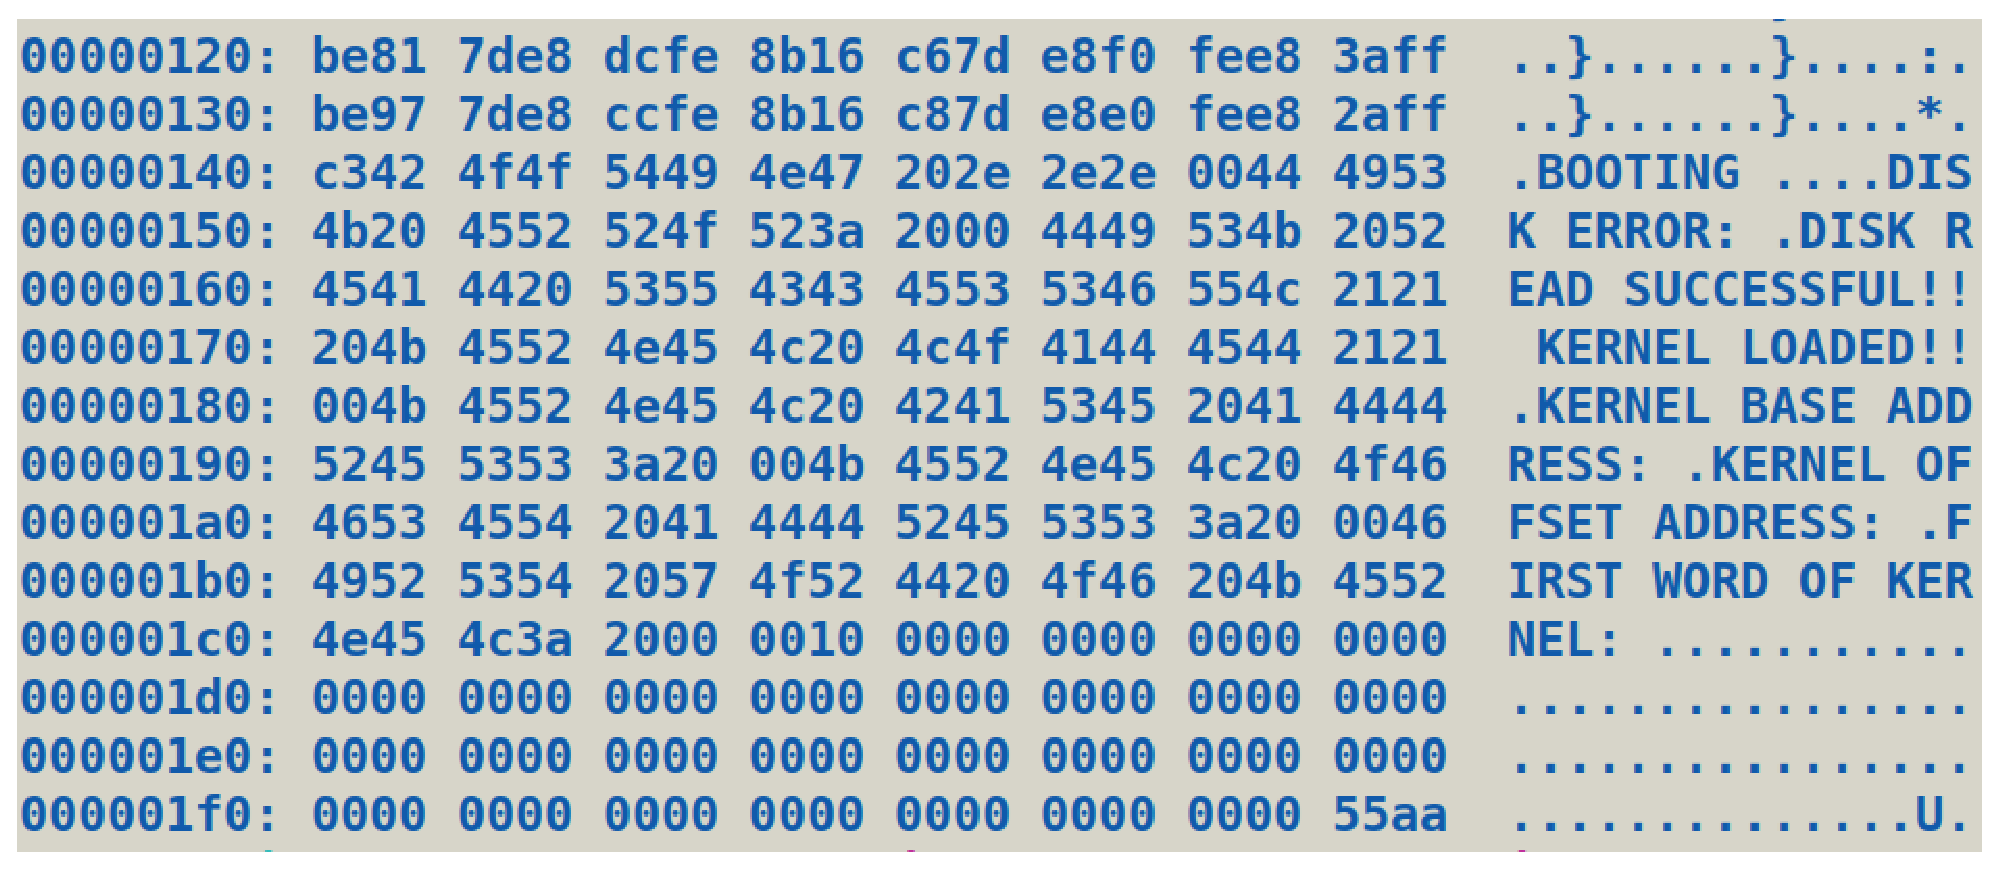
\includegraphics[scale=0.30]{figures/boothexdump.eps}
  \caption{Hexdump of the bootloader showing the placement of the magic number 0xaa55}
\label{fig:boothexdump}
\end{figure}

\subsection{boot\_util.asm}
It is important to print a few messages on the screen when the bootloader is loading the operating system. These messages especially useful in the event disk read operation has failed and the kernel has not been loaded properly. To print such messages, we make use of INT 10,0E which allows us to print characters to the screen in teletype mode. The subroutines used by the bootloader to which to print strings, newlines and hexadecimal numbers on the screen are present in \texttt{boot\_util.asm} file. These were some of the first subroutines which were developed as part of this project. These are:
\begin{enumerate}
  \item \texttt{print}
  		\begin{enumerate}[align=parleft, labelsep=2cm, leftmargin=1.06in]
  		  \item[Input]: \verb|si| = pointer to the first byte of a string
  		  \item[Output]: Nothing\footnote[1]{In context of a subroutine, the term "output" means the value that is being returned by it.}
  		  \item[Description]: Prints a null (0x00) terminated string pointed at by \verb|si|.
  		\end{enumerate}
  \item \texttt{printhex}
  		\begin{enumerate}[align=parleft, labelsep=2cm, leftmargin=1.06in]
  		  \item[Input]: \texttt{dx} = 16-bit hexadecimal number
  		  \item[Output]: Nothing
  		  \item[Description]: Prints the hexadecimal number stored in \verb|dx| in \texttt{0x\_\_\_\_} format. Uses right-shift operation \texttt{shr} and logical AND, \texttt{and}, to decompose the hexadecimal number stored in \verb|dx| into individual nibbles. A string representing the hexadecimal number is then made by adding each individual nibble to the ASCII value of either '0' or 'A' depending upon the whether it is less than 0x0a or not, respectively. The string is then printed using \texttt{print} subroutine.
  		\end{enumerate} 
  \item \texttt{printnl}
  		\begin{enumerate}[align=parleft, labelsep=2cm, leftmargin=1.06in]
  		  \item[Input]: Nothing
  		  \item[Output]: Nothing
  		  \item[Description]: Prints a newline, i.e., positions cursor at the beginning of the next line. This is achieved by printing line-feed character (0x0a) and carriage return (0x0d) using INT 10,0E. This is equivalent to \texttt{printf("\textbackslash n");} used in C programs for positioning the cursor at the beginning of the next line.
  		\end{enumerate}
\end{enumerate}

\section{Kernel Header: ../kernel/kernel.asm}
If one were to draw a memory map for CrazyOS (\autoref{fig:osmemmap}), they will find that the subroutine which is placed at the lowest memory address is the \texttt{kernel\_entry} subroutine. The operating system can be said to begin with this subroutine.
\begin{figure}[h]
  \centering
  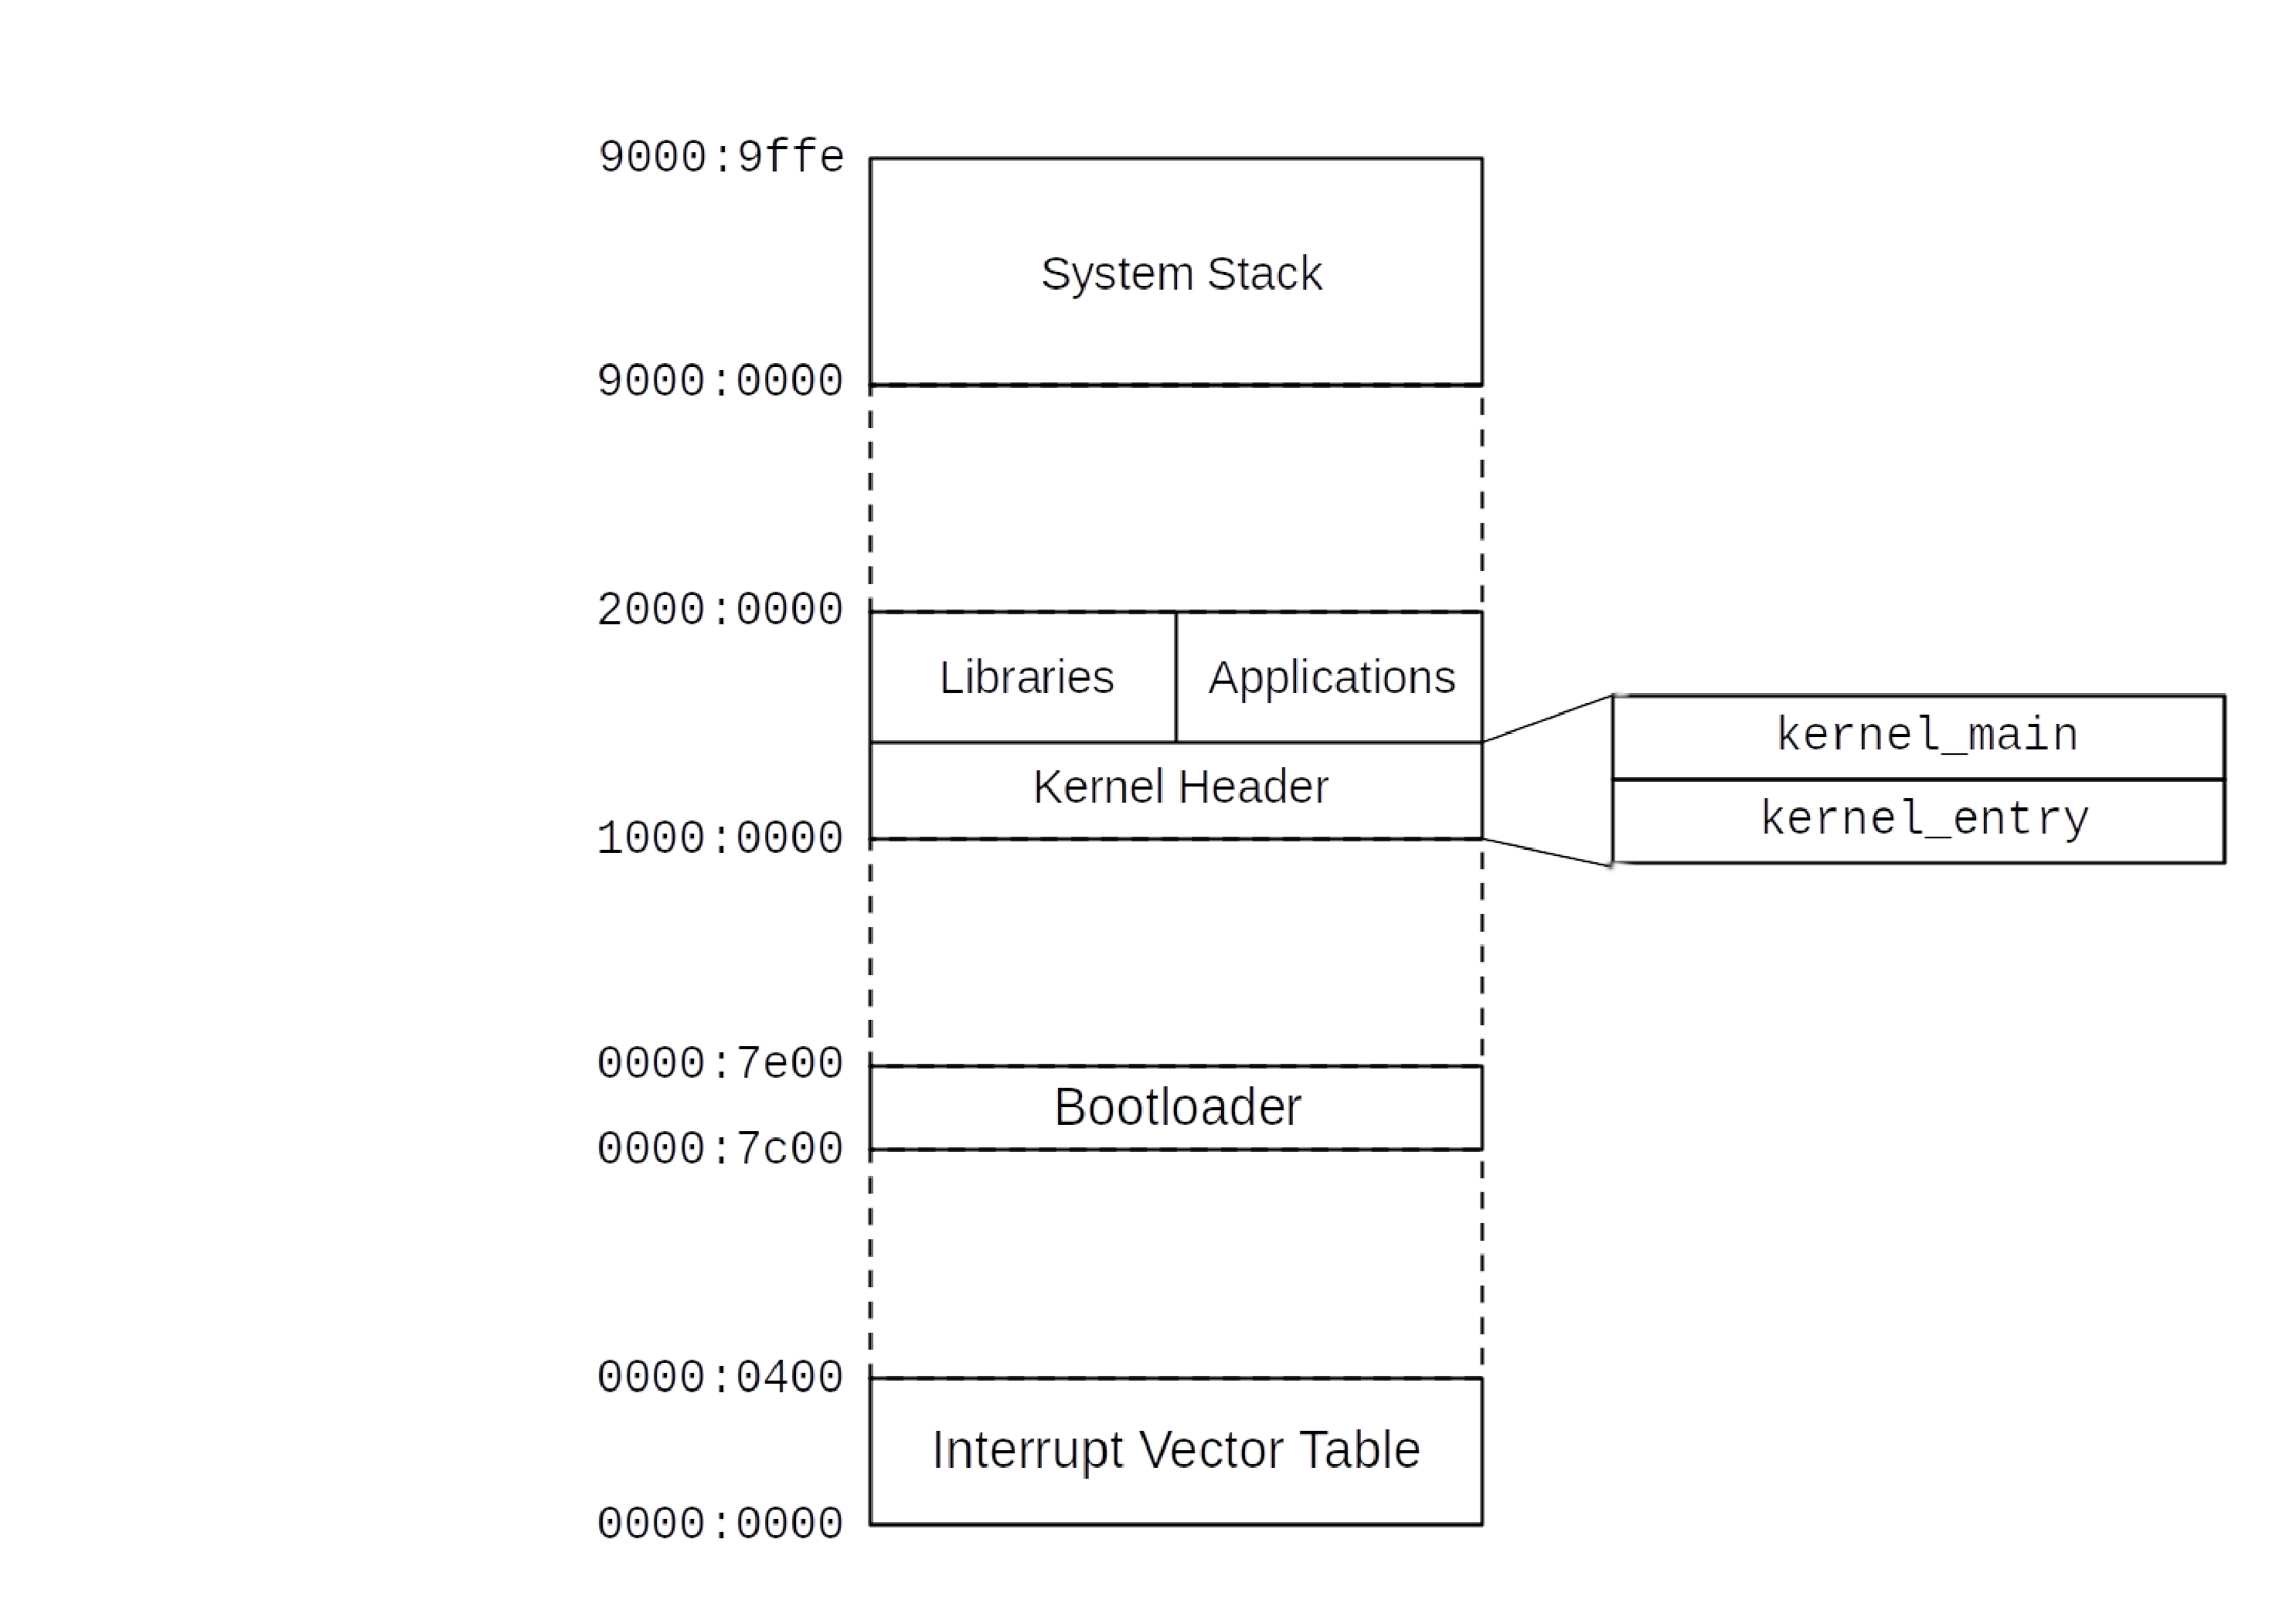
\includegraphics[scale=0.25]{figures/osmemmap.eps}
  \caption{Memory map of CrazyOS}
\label{fig:osmemmap}
\end{figure}
If \texttt{kernel.asm} forms the head of the operating system, then \texttt{kerne\_entry} subroutine would be the scalp and \texttt{kernel\_main} would be the cranium of the operating system. The bootloader performs an intersegment call to \textit{kernel\_entry} subroutine which has been loaded, along with the rest of the operating system, in block 1. \texttt{kernel\_entry} subroutine is responsible for initializing \texttt{cs}, \texttt{ds}, \texttt{es}, and \texttt{ss}.
\begin{Verbatim}
kernel_entry:
	mov ax, cs
	mov ds, ax
	mov es, ax
	mov ax, 0x9000
	mov ss, ax
	mov bp, 0x9ffe
	mov sp, bp
\end{Verbatim}
After an intersegment call has been performed by the bootloader, \texttt{cs} has been loaded with 0x1000. \verb|ds| and \verb|es| should also use the same base address as the data for the operating system has also been loaded in block 1 itself. As we cannot assign a value to segment registers directly, therefore, we store the value in \verb|cs| in \verb|ax|. Then the value stored in \verb|ax| is assigned to \verb|ds| and \verb|es|. Furthermore, we must make sure that our stack is not in the same segment as the code and data segments, otherwise problems will occur if \verb|sp| and \verb|bp| start pointing at data and instruction words. That is why the stack for the operating system is formed in block 9 which is far away from block 1. \verb|ss| is initialized with a value of 0x9000, and \verb|bp| and \verb|sp| with a value of 0x9ffe.\\
\texttt{kernel\_main} subroutine begins just after \texttt{kernel\_entry} subroutine. It is analogous to the \texttt{while(1) \{ } loop which is an infinite loop which runs a sequence of tasks again and again. \texttt{kernel\_main} clears the screen, prints a test message, date and time, and then call the \texttt{main} subroutine present in \texttt{../apps/shell.asm}.

\section{Library Functions: ../include}

\begin{figure}
\begin{forest}
  for tree={
    font=\ttfamily,
    grow'=0,
    child anchor=west,
    parent anchor=south,
    anchor=west,
    calign=first,
    edge path={
      \noexpand\path [draw, \forestoption{edge}]
      (!u.south west) +(7.5pt,0) |- node[fill,inner sep=1.25pt] {} (.child anchor)\forestoption{edge label};
    },
    before typesetting nodes={
      if n=1
        {insert before={[,phantom]}}
        {}
    },
    fit=band,
    before computing xy={l=15pt},
  }
[CrazyOS/8086/include
  [apm
    [apm\_com.asm]
    [apm.asm]
  ]
  [cmos
    [cmos\_com.asm]
    [cmos.asm]
  ]
  [disk
    [disk\_com.asm]
    [disk.asm]
  ]
  [random
    [srng.asm]
  ]
  [sound
    [sound.asm]
  ]
  [string
    [lexer.asm]
    [README.txt]
    [string.asm]
  ]
  [ttyio
    [legacyprint.asm]
    [printf.asm]
    [README.txt]
    [stdtty.asm]
    [ttyio.asm]  
  ]
]
\end{forest}
\caption{Directory tree for \texttt{CrazyOS/8086/include} (depth = 1)}
\label{fig:dirtc8include}
\end{figure}

Every operating system comes with a bunch of subroutines which are used by applications to interact with the hardware. Subroutines using which other subroutines can be built are called system calls. System calls can be issued by either calling the subroutine, or by issuing a software interrupt in the same manner a BIOS interrupt call is used to invoke the facilities provided by the BIOS. System calls and other such fundamental functions are kept in a separate directory, usually protected from user's tampering. These functions are often called library functions. In CrazyOS, these library functions are placed in \texttt{../8086/include} folder. Source tree of this directory is shown in \autoref{fig:dirtc8include}. As these functions use BIOS calls to access hardware facilities, the reader can think of BIOS interrupts as system calls. The subroutines present in the library are analogous to functions present in the standard C library such as \texttt{printf}, \texttt{scanf}, \texttt{atoi}, etc., which a programmer often uses in their application to get the job done.\\
Some of the library functions present in this directory were inspired by the standard C library functions. The rest were created as and when the need for accessing a specific piece of hardware was required. We will describe each these functions beginning with the ones which took inspiration from their standard C library counterparts. Before explaining these library functions, we will explain the organization of library files, and the \texttt{include} guard.

\subsection{Organization of Library Functions}
The first few subroutines in the library used to deal with setting up a terminal environment and handling strings. Later on, the author started dealing with device specific codes and also wrote subroutines which were executed when a command was entered in the shell. This prompted the author to organize the \texttt{../include} folder. Each subfolder in  \texttt{../include} deals with a particular component of the computer or some process. The name of the subfolder is same as the name of the device it deals with. Baring a few exceptions, subfolders present in the library contain two types of files:
\begin{enumerate}
  \item \textit{Fundamental files}: As the name speaks for itself, these files contain core subroutines which deal with devices making up the system. These subroutines might be present in different files, but are always clubbed together into a single file having the same name as that of the folder it is present in. For example, the subroutines dealing with setting up a terminal environment are present in different source files in \texttt{../include/ttyio} subdirectory, but are clubbed together into a single file named \texttt{ttyio.asm}.
  \item \textit{Command processing files}: These files contain subroutines which are executed in response to commands that has been entered in the shell. These subroutines often make use of subroutines present in fundamental files present in the same or other directories. These files also bear the same name as the folder they are present in, but have the suffix \texttt{\_com} added to them. For example, the fundamental procedures dealing with disk operations are kept in \texttt{../include/disk/disk.asm} and those procedures which are executed in response to entering of disk read/write commands in the shell are kept in \texttt{../include/disk/disk\_com.asm} file.
\end{enumerate}

\subsection{\%include Guard}
In C language, the C preprocessor processes statements which begin with \texttt{\#}. These statements are called preprocessor directives. Examples are \texttt{\# include} and \texttt{\# define} directives. The \texttt{\# include} directive is followed by the name of a file whose functions are being used in the current file. The preprocessor expands the contents of the file in place of the directive. As the size of a project grows, so does the number of source files. Including the same file more than once can cause problems during the linking stage as the linker will get confused by the multiple occurrences of the same label in different object files. To prevent such problems, The file to be included has its contents placed in between \texttt{\# ifndef}, \texttt{\# define}, and \texttt{\# endif} directives. These are called \texttt{include} guard, as they ensure that if a macro has already been declared, then there is no need to include the contents of the header file again in the final binary. For example, the first two statements of \texttt{stdio.h} file are
\begin{Verbatim}
#ifndef _STDIO_H
#define _STDIO_H		1
\end{Verbatim}
and its last statement is
\begin{Verbatim}
#endif			/* <stdio.h> included.  */
\end{Verbatim}
The contents of \texttt{stdio.h} are included between these statements. This way a programmer can include the files they think are necessary for a project and not worry about repeated inclusion of files.\\
NASM provides us with \texttt{\%ifndef}, \texttt{\%define}, and \texttt{\%endif} directives which work exactly like their C counterparts. Library subroutines often use this guard to ensure that no assembly source file is included more than once in the final binary of the project. As an example, the first few lines of \texttt{../include/ttyio/ttyio.asm} are
\begin{Verbatim}
bits 16
align 16
%ifndef TTYIO
%define TTYIO
%include "include/ttyio/legacyprint.asm"
%include "include/ttyio/printf.asm"
%include "include/ttyio/stdtty.asm"
\end{Verbatim}

and its closing line is
\begin{Verbatim}
%endif
\end{Verbatim}

\subsection{Standard I/O subroutines: ../include/ttyio}
A programmer just needs to include \texttt{ttyio.asm} file in his source file to get access to all the functions which are available for printing on the screen and for taking input from the keyboard. The file \texttt{ttyio.asm} contains a single subroutine, \texttt{fstringdata}, with the rest coming from inclusion of \texttt{legacyprint.asm}, \texttt{printf.asm}, and \texttt{stdtty.asm}. \texttt{fstringdata} can be described as follows:
\begin{enumerate}
  \item[]\texttt{fstringdata}
\begin{enumerate}[align=parleft, labelsep=2cm, leftmargin=1.5in]
  		  \item[Input]: \texttt{si} = pointer to a null terminated string, \newline\texttt{ax} = data to be entered,\newline\texttt{cx} = position at which data is to be entered
  		  \item[Output]: Nothing 
  		  \item[Description]: Used to enter data next to a null-terminated formatted string.
  		\end{enumerate}
\end{enumerate}
\texttt{legacyprint.asm} was the first library file which was written for this project. Two functions, namely, \verb|print|, and \texttt{printnl}, have been directly copied from \texttt{../boot/boot\_util.asm}. \texttt{printhex} subroutine present in this file bears the same name as its counterpart which was used in the bootloader to print hexadecimal numbers. However, this version of \texttt{printhex} uses right rotation instruction, \verb|ror|, to decompose the 16-bit hexadecimal number stored in \textbf{\texttt{ax}} into nibbles. Other functions which have been included in this file are: 
\begin{enumerate}
  \item \texttt{print8bitpackedBCD}
  		\begin{enumerate}[align=parleft, labelsep=2cm, leftmargin=1.06in]
  		  \item[Input]: \texttt{ah} = 0x00,\newline\texttt{al} = 8-bit packed BCD
  		  \item[Output]: Nothing
  		  \item[Description]: Prints an 8-bit packed BCD stored in \texttt{al}.
  		\end{enumerate}
  \item \texttt{printdec}
  		\begin{enumerate}[align=parleft, labelsep=2cm, leftmargin=1.06in]
  		  \item[Input]: \texttt{ax} = 16-bit number (0 - 65535)
  		  \item[Output]: Nothing
  		  \item[Description]: Prints a 16-bit number stored in \texttt{ax} in decimal format. A blank space is printed if the number is equal to 0.
  		\end{enumerate}
\end{enumerate}
\texttt{stdtty.asm} defines several subroutines which enable the user to print characters on the screen as well as take input from the keyboard. The functions defined in this source file are:
\begin{enumerate}
  \item \texttt{clear}
  		\begin{enumerate}[align=parleft, labelsep=2cm, leftmargin=1.06in]
  		  \item[Input]: Nothing
  		  \item[Output]: Nothing
  		  \item[Description]: Similar to the working of \texttt{clrscr} subroutine in \texttt{../boot/boot.asm}, this subroutine clears the screen, sets page-number to 0, resets background and foreground colour to their default values, and positions the cursor at row 0 and column 0. Executed when \texttt{clear} command is entered in the shell.
  		\end{enumerate}
  \item \texttt{findcursorposition}
  		\begin{enumerate}[align=parleft, labelsep=2cm, leftmargin=1.06in]
  		  \item[Input]: Nothing
  		  \item[Output]: \texttt{dh} = row at which the cursor is positioned (0 - 24),\newline\texttt{dl} = column at which the cursor is positioned (0 - 79)
  		  \item[Description]: Used to find the position of the cursor. 
  		\end{enumerate}
  \item \texttt{scrollup}
  		\begin{enumerate}[align=parleft, labelsep=2cm, leftmargin=1.06in]
  		  \item[Input]: Nothing
  		  \item[Output]: Nothing
  		  \item[Description]: Scrolls the screen up by a single line only
  		\end{enumerate}
  \item \texttt{conditional\_scrollup}
  		\begin{enumerate}[align=parleft, labelsep=2cm, leftmargin=1.06in]
  		  \item[Input]: Nothing
  		  \item[Output]: Nothing
  		  \item[Description]: Finds the position of the cursor and scrolls the screen up by a single line if the cursor is found to be positioned at the 24th row.
  		\end{enumerate}
  \item \texttt{putchar}
  		\begin{enumerate}[align=parleft, labelsep=2cm, leftmargin=1.06in]
  		  \item[Input]: \texttt{al} = code of the character to be printed from code page 437
  		  \item[Output]: Nothing
  		  \item[Description]: Prints a single character onto the screen. Calls \texttt{conditional\_scrollup} and \texttt{printnl} to scroll the screen up by one line in case the cursor is at 24th row.
  		\end{enumerate}
  \item \texttt{getchar}
  		\begin{enumerate}[align=parleft, labelsep=2cm, leftmargin=1.06in]
  		  \item[Input]: Nothing
  		  \item[Output]: \texttt{ah} = keyscan code of the key combination that has been pressed, \texttt{al} = code of the character corresponding to the key combination that has been pressed. 
  		  \item[Description]: Reads a key from the keyboard and returns the corresponding key scan codes and character code in \texttt{ah} and \texttt{al}, respectively.
  		\end{enumerate}
  \item \texttt{getline}
  		\begin{enumerate}[align=parleft, labelsep=2cm, leftmargin=1.06in]
  		  \item[Input]: Nothing
  		  \item[Output]: \texttt{si} = pointer to the 80-byte wide buffer, \texttt{GETLINE\_BUFFER}
  		  \item[Description]: Allows the user to input a single line, having a maximum length of 80 characters, through the keyboard. Printable ASCII characters are printed on the screen. Rest of the characters perform control sequence such as deleting a character, positioning the cursor, etc. Not all cursor control sequences are supported. \texttt{si} is returned as a pointer to the \texttt{GETLINE\_BUFFER}.
  		\end{enumerate}
  \item \texttt{flush}
  		\begin{enumerate}[align=parleft, labelsep=2cm, leftmargin=1.06in]
  		  \item[Input]: Nothing
  		  \item[Output]: Nothing
  		  \item[Description]: Flushes the \texttt{GETLINE\_BUFFER} by setting all 80 bytes it is made up of equal to 0x00.
  		\end{enumerate}
\end{enumerate}
Finally, we come to \texttt{printf.asm} which has the source code for a bare-minimum implementation of \texttt{printf} found in C.
\begin{enumerate}
  \item[]\texttt{printf}
  		\begin{enumerate}[align=parleft, labelsep=2cm, leftmargin=1.06in]
  		  \item[Input]: \texttt{si} = pointer to a null-terminated string followed by optional data to be printed.
  		  \item[Output]: Nothing
  		  \item[Description]: A bare-minimum implementation of \texttt{printf}. Data which is to be printed should have word size and should be entered after terminating null word of the string using \texttt{fstringdata} subroutine. Supported format specifiers are:
  		  \begin{enumerate}[align=parleft, labelsep=2cm]
  		    \item[]\verb|%c|: Single character
  		    \item[]\verb|%d|: 16-bit number in decimal format
  		    \item[]\verb|%x|: 16-bit number in hexadecimal format
  		  \end{enumerate}
Supported escape sequences are:
  		  \begin{enumerate}[align=parleft, labelsep=2cm]
  		    \item[]\verb|\n|: Newline
  		    \item[]\verb|\t|: Tab
  		  \end{enumerate}
  		\end{enumerate}
\end{enumerate}

\subsection{String Handling: ../include/string}
String handling is an important part of any language. The programmer who is writing applications for CrazyOS has to include \texttt{../include/string/string.asm} in his application program to allow him to use various subroutines to handle strings. These subroutines have been inspired from their counterparts found in \texttt{string.h} in C. These subroutines have been described below:
\begin{enumerate}
  \item \texttt{strlen}
  		\begin{enumerate}[align=parleft, labelsep=2cm, leftmargin=1.06in]
  		  \item[Input]: \texttt{si} = pointer to a null-terminated string
  		  \item[Output]: \texttt{ax} = length of the string pointed at by \texttt{si}
  		  \item[Description]: Used to compute the length of the string.
  		\end{enumerate}
  \item \texttt{strcmp}
  		\begin{enumerate}[align=parleft, labelsep=2cm, leftmargin=1.06in]
  		  \item[Input]: \texttt{si} = pointer to the first null-terminated string,\newline\texttt{di} = pointer to the second null-terminated string
  		  \item[Output]: \texttt{ax} = 0x00 if the the strings are equal, or\newline\texttt{ax} = 0x01 if the strings are not equal
  		  \item[Description]: Compares two strings which are being pointed at by \texttt{si} and \texttt{di}. It first compares their length using \texttt{strlen} subroutine. If the lengths are found to be equal, it then compares them character by character. If both the strings are found to be equal to each other, then \texttt{ax} is returned with 0x00, else \texttt{ax} is set to 0x01
  		\end{enumerate}
  \item \texttt{strcpy}
  		\begin{enumerate}[align=parleft, labelsep=2cm, leftmargin=1.06in]
  		  \item[Input]: \texttt{si} = pointer to the null-terminated source string,\newline\texttt{di} = pointer to the destination string
  		  \item[Output]: Nothing
  		  \item[Description]: Copies the source string pointed at by \texttt{si} to the destination string pointed at by \texttt{di}. \texttt{rep movsb} instruction is used to perform this copying operation.
  		\end{enumerate}
  \item \texttt{atoi}
  		\begin{enumerate}[align=parleft, labelsep=2cm, leftmargin=1.06in]
  		  \item[Input]: \texttt{si} = pointer to the string representation of a 16-bit positive number.
  		  \item[Output]: \texttt{ax} = number which was stored in the string pointed at by \texttt{si}
  		  \item[Description]: Converts the string representation of a number to a 16-bit number, stores it in \texttt{ax}, and returns to the caller.
  		\end{enumerate}
  \item \texttt{atoh}
  		\begin{enumerate}[align=parleft, labelsep=2cm, leftmargin=1.06in]
  		  \item[Input]: \texttt{si} = pointer to the string representation of a hexadecimal number
  		  \item[Output]: \texttt{ax} = hexadecimal number which was stored in string format
  		  \item[Description]: Converts the string representation of a hexadecimal number, stores it in \texttt{ax}, and returns to the caller. Although the prefix "0x" is used when printing hexadecimal numbers, it should be made sure that the string being passed to atoh does not have this prefix.
  		\end{enumerate}
\end{enumerate}

\texttt{..include/string} directory has another assembly source file besides \texttt{string.asm}. It is \texttt{lexer.asm} which is responsible for breaking a string of characters into separate "words" using some separator. The function used for performing this primitive lexical-analysis is \texttt{cmd\_lexer}. Its description is given below:
\begin{enumerate}
  \item[] \texttt{cmd\_lexer}
  		\begin{enumerate}[align=parleft, labelsep=2cm, leftmargin=1.06in]
  		  \item[Input]: \texttt{al} = ASCII code of the character to be used as a separator,\newline\texttt{si} = pointer to the 80-byte wide string
  		  \item[Output]: Nothing
  		  \item[Description]: \textit{Tokenizes} the string that is being pointed at by \texttt{si} using the character stored in \texttt{al} as a separator. It generates its own personal copy of the string which is stored in local label \texttt{.COPY}. This subroutine is capable of generating a maximum of 5 tokens: one command token and four argument tokens. Command token is stored in global label \texttt{com} and argument tokens are stored in \texttt{arg1}, \texttt{arg2}, \texttt{arg3}, and \texttt{4} which are also global labels.
  		\end{enumerate}
\end{enumerate} 
\subsection{CMOS and RTC: ..include/cmos}
Real time clock, or RTC for short, is responsible for keeping track of date and time even when the computer has been turned off. This is achieved by independently powering the RTC using a CR2032 coin cell. As the power consumption of RTC is very small, one coin cell lasts for many years. The RTC chip also has very low power static CMOS memory. Although the term CMOS specifically refers to a type of semiconductor technology, when used in context with personal computers, the term refers to the static memory on the RTC chip. This memory has several registers which store setup information for the BIOS even when the computer is turned off. The first 14 CMOS registers store the time and date and control the operation of the RTC. CMOS registers can be accessed using \verb|in| and \verb|out| instructions. CMOS's input is mapped to port 0x70 and its output is mapped to 0x71. Before writing anything to these ports the interrupts must be disabled using \verb|cli|. They can later be enabled using \verb|sti|. To read the value of a CMOS register, we store the register number in \verb|al| and then execute the following instructions:
\begin{Verbatim}
        cli
        out 0x70, al
        nop
        in al, 0x71
        sti
\end{Verbatim}
The value of the register is returned in \verb|al|. To write a value to a CMOS register, we first select the register by passing its number to port 0x70. Then write the value to be written at port 0x71. The code for the same is shown below:
\begin{Verbatim}
        cli
        out 0x70, al
        nop
        mov al, bl 
        out 0x71, al
        sti
\end{Verbatim}
Simple subroutines to read and write CMOS registers are kept in \texttt{cmos.asm} file. These subroutines are:
\begin{enumerate}
  \item \texttt{read\_cmos}
  		\begin{enumerate}[align=parleft, labelsep=2cm, leftmargin=1.06in]
  		  \item[Input]: \texttt{al} = index of the register to be accessed
  		  \item[Output]: \texttt{al} = value of the register that was accessed
  		  \item[Description]: Used to read the value of a register. Interrupts are disabled before executing port I/O instructions and are enabled before returning to the caller. A \texttt{nop} instruction is executed between two consecutive port operations. This gives the system enough time to perform port operation correctly.
  		\end{enumerate}
  \item \texttt{write\_cmos}
  		\begin{enumerate}[align=parleft, labelsep=2cm, leftmargin=1.06in]
  		  \item[Input]: \texttt{al} = index of the register to be accessed,\newline\texttt{bl} = value to be written to the register
  		  \item[Output]: Nothing
  		  \item[Description]: Writes a value passed in \texttt{bl} to the CMOS register with index equal to the value stored in \texttt{al}.
  		\end{enumerate}
\end{enumerate}
\texttt{cmos\_com.asm} contains subroutines which are executed when \texttt{date} or \texttt{time} commands are entered in the shell. These subroutines are:
\begin{enumerate}
  \item \texttt{time}
  		\begin{enumerate}[align=parleft, labelsep=2cm, leftmargin=1.06in]
  		  \item[Input]: Nothing
  		  \item[Output]: Nothing
  		  \item[Description]: Global variables \texttt{HRS}, \texttt{MIN}, and \texttt{SEC} are updated with the value of hour, minutes, seconds at the time of execution of the function, respectively.
  		\end{enumerate}
  \item \texttt{showtime}
  		\begin{enumerate}[align=parleft, labelsep=2cm, leftmargin=1.06in]
  		  \item[Input]: Nothing
  		  \item[Output]: Nothing
  		  \item[Description]: Prints time in \texttt{HH:MM:SS} format. Hour is printed in 24-hour format. Executed when \texttt{time} command is entered in the shell.
  		\end{enumerate}
  \item \texttt{date}
  		\begin{enumerate}[align=parleft, labelsep=2cm, leftmargin=1.06in]
  		  \item[Input]: Nothing
  		  \item[Output]: Nothing
  		  \item[Description]: Global variables \texttt{WEEKDAY}, \texttt{DAY\_OF\_THE\_MONTH}, \texttt{MONTH}, and \texttt{YEAR} are updated with the value of current index of weekday (Sunday = 1, Monday = 2, etc.), day of the month, month number, and last two digits of the year at the time of execution of the function, respectively.
  		\end{enumerate}
  \item \texttt{showdate}
  		\begin{enumerate}[align=parleft, labelsep=2cm, leftmargin=1.06in]
  		  \item[Input]: Nothing
  		  \item[Output]: Nothing
  		  \item[Description]: Displays current date in \texttt{Weekday, DD-MM-YY} format. Executed when \texttt{date} command is entered in the shell.
  		\end{enumerate}
\end{enumerate}

\subsection{Random Number Generator: ../include/random}
Random number generators often find application in games, cryptography, and computer simulation. The author has written a simple pseudo-random number generator, \texttt{srng}. It is described as follow:
\begin{enumerate}
  \item[]\texttt{srng}
  		\begin{enumerate}[align=parleft, labelsep=2cm, leftmargin=1.06in]
  		  \item[Input]: Nothing 
  		  \item[Output]: \texttt{ax} = pseudo-random number
  		  \item[Description]: Produces a pseudo-random number by taking the value of seconds elapsed as a seed value. This value is obtained from register 0x00 of the CMOS. This seed value is multiplied with 8999d, which is a prime number. 9923d, which is another prime number, is added to the product's low byte to produce a pseudo-random number which is returned in \texttt{ax}. 
  		\end{enumerate}
\end{enumerate}

\subsection{Sound Generator: ../include/sound}
Before discussing the process of sound generation in an IBM PC, we must briefly discuss the 8254 programmable interval timer (PIT) chip. This chip was primarily designed to solve timing control problems in microcomputers. Its block diagram is shown in \autoref{fig:8254}.

\begin{figure}[h]
  \centering
  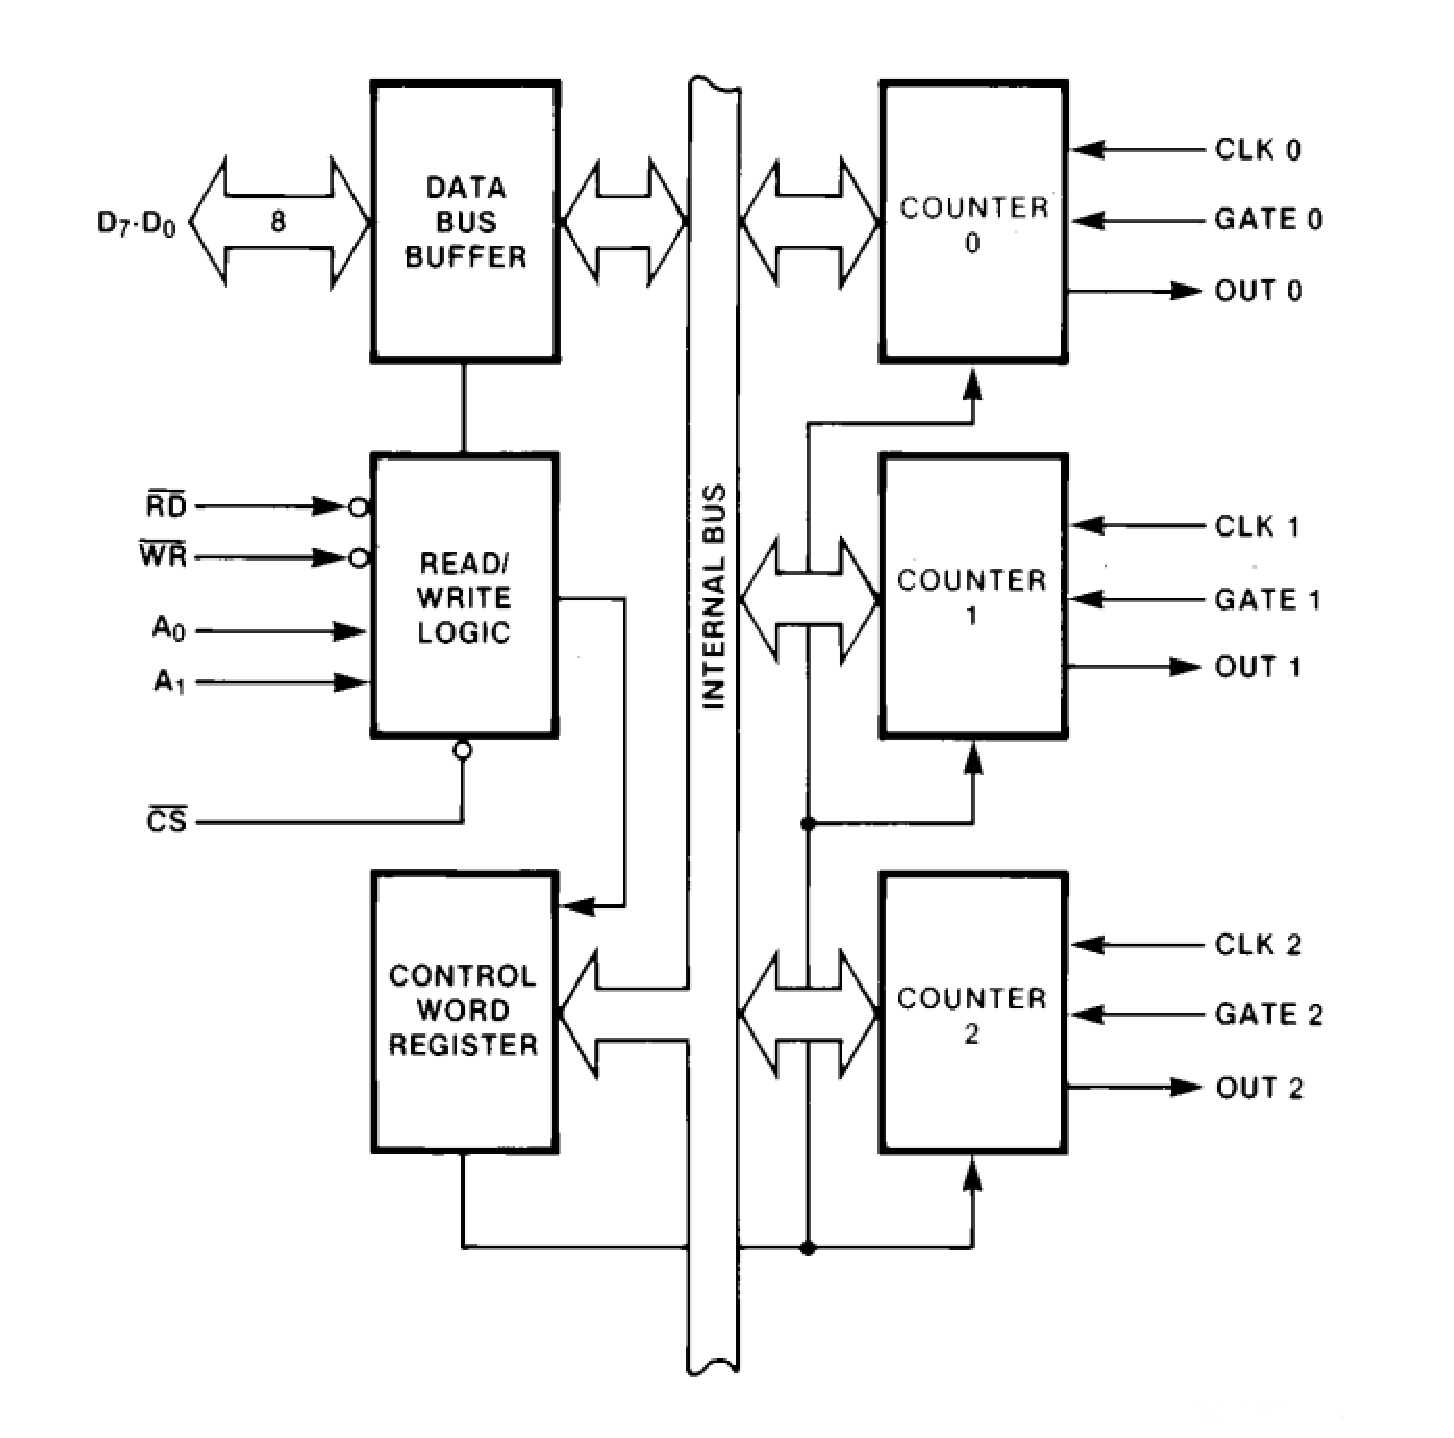
\includegraphics[scale=0.30]{figures/8254.eps}
  \caption{Block diagram of the 8254 PIT chip \cite{intel1993PIT}}
\label{fig:8254}
\end{figure}

It consists of 3 counters/timers, each capable of working independently of each other. Numbering of timers start from 0. Therefore, we have timer 0, timer 1, and timer 2. The mode in which each timer operates is decided by the value which has been passed to the control word register. The format of the word which is passed on to the control word register is shown in \autoref{fig:8254cwr}. On an IBM PC, control word register is mapped to port 0x43. Once the control word has been transmitted, the counter of each timer needs to be initialized with some value. Count down starts from this value. The counters of timers are also mapped to I/O ports starting from port 0x40. So, timer 0's counter is mapped to port 0x40, timer 1's counter is mapped to port 0x41, and timer 2's counter is mapped to port 0x42. Each timer/channel two input pins, namely \texttt{CLK} and \texttt{GATE}. The former receives clock signal from an oscillator running at approximately 1.19 MHz. The later is used to enable an output signal from the output pin, \texttt{OUT} \cite{intel1993PIT}.

\begin{figure}[h]
  \centering
  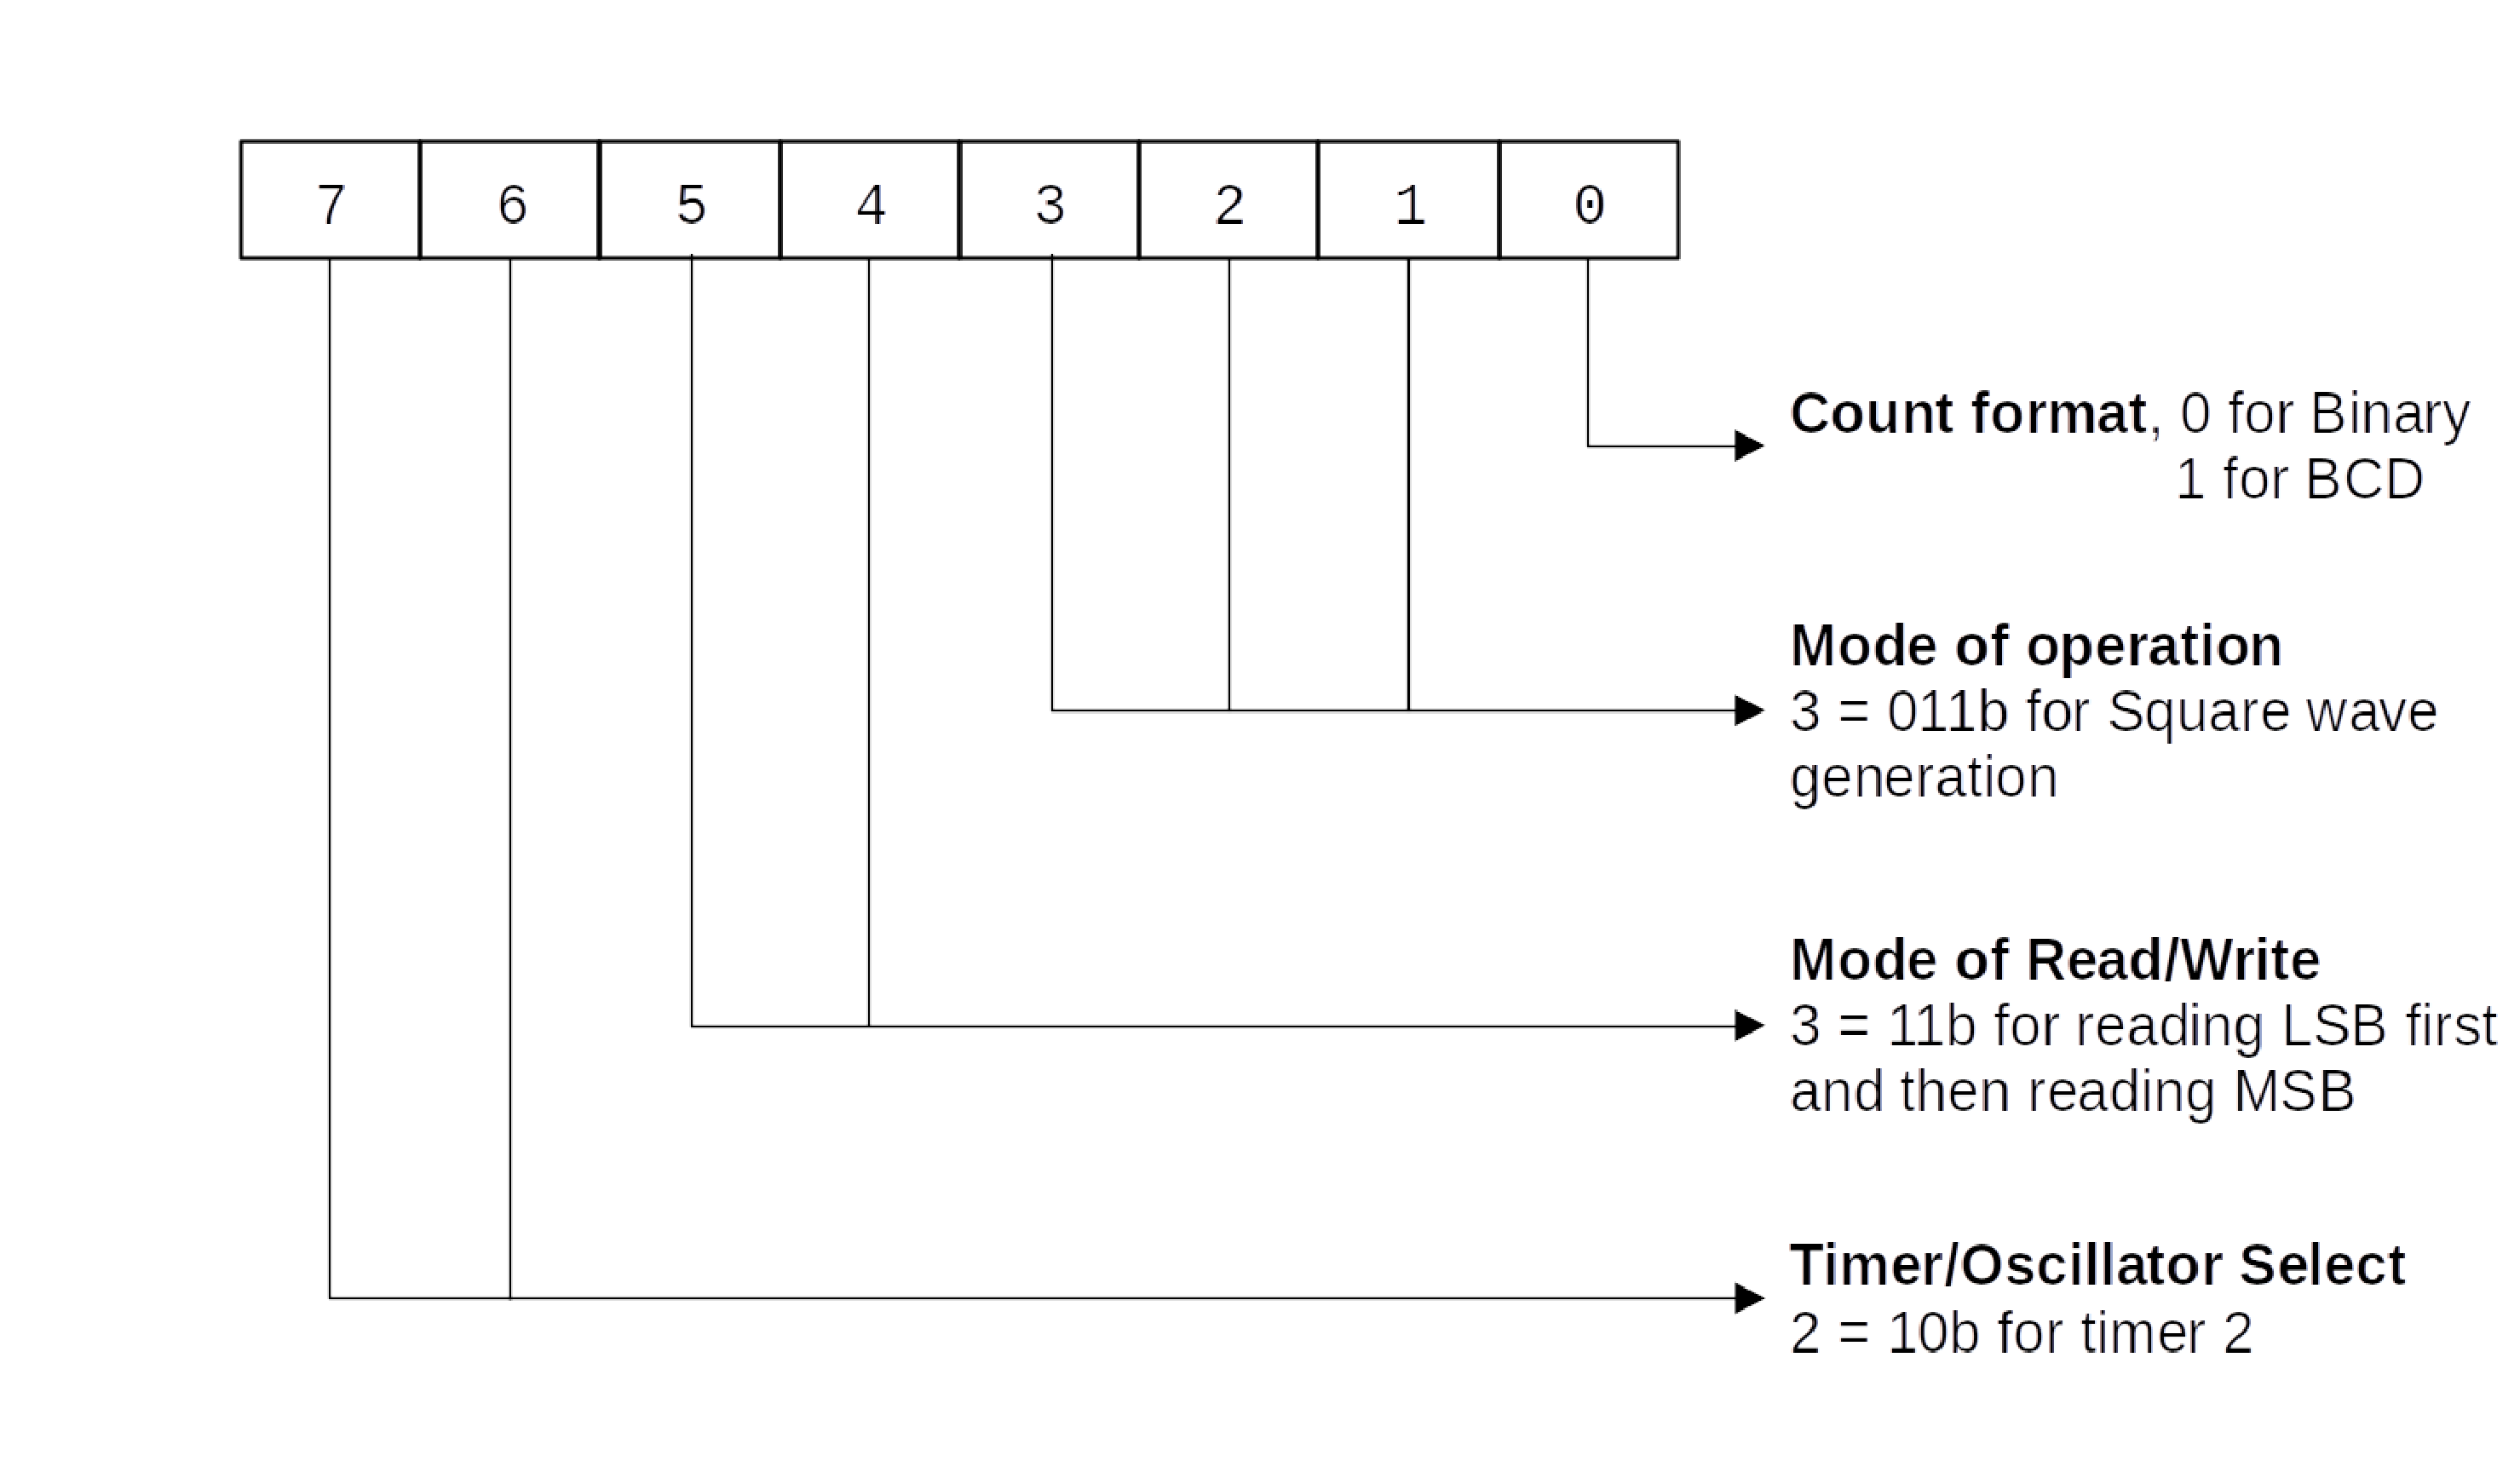
\includegraphics[scale=0.25]{figures/8254cwr.eps}
  \caption{Control word format for the PIT chip}
\label{fig:8254cwr}
\end{figure}

We are interested in operating the piezoelectric speaker which is soldered onto the motherboard of PCs. This piezoelectric speaker is driven by the signal generated by timer 2, and is connected to its \texttt{OUT} line using an AND gate as shown in \autoref{fig:speakermap}. The second pin of this AND gate is mapped to bit 1 of port 0x61. \texttt{GATE 2} pin is mapped to bit 0 of port 0x61.

\begin{figure}[h]
  \centering
  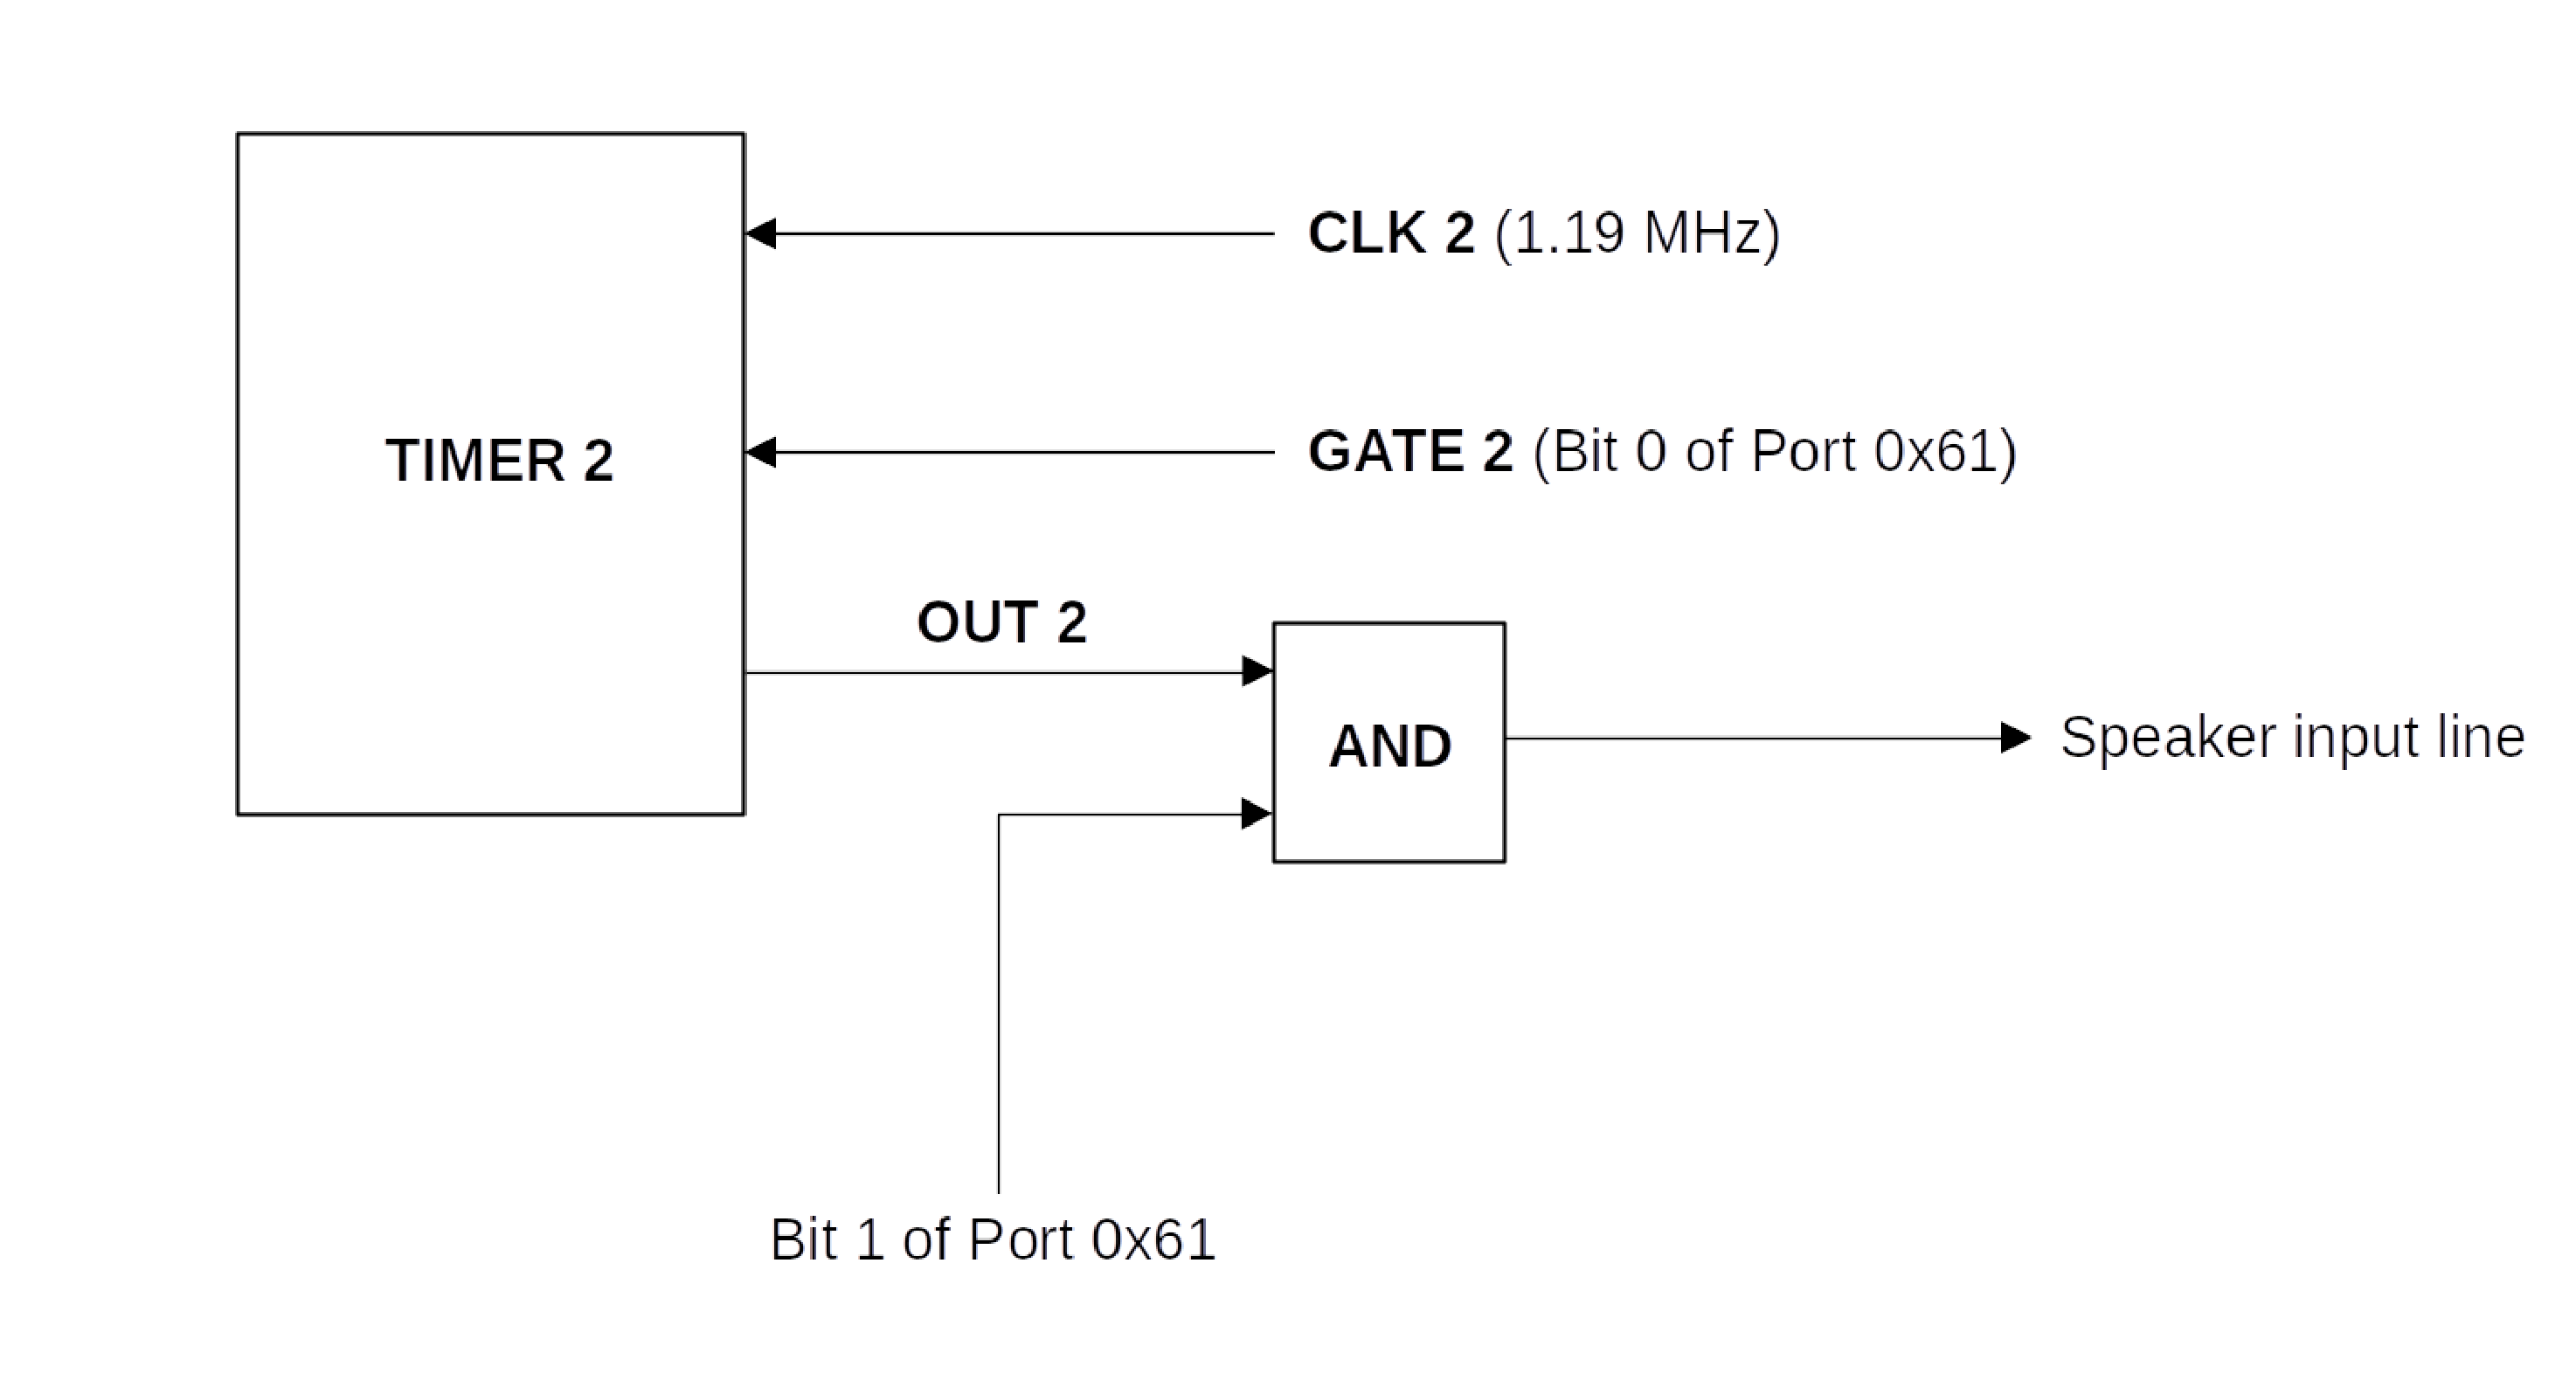
\includegraphics[scale=0.25]{figures/speakermap.eps}
  \caption{Connection of motherboard speaker with timer 2 of the PIT chip}
\label{fig:speakermap}
\end{figure}

The algorithm for producing a sound from the speaker by generating a square wave of particular frequency from timer 2 is as follows:
\begin{steps}[leftmargin=2cm]
  \item Select the frequency, $f$, of the sound you wish to generate. 
  \item Compute the value to be stored in the counter using the following formula:
  \begin{center}
  Value to be stored in the the counter, $N = \frac{1.19 MHz}{f}$
  \end{center}
  \item Round of $N$ to the nearest integer.
  \item Output a byte to port 0x43 specifying that timer 2 is to be used as a square wave generator, with the value of latch count being transmitted in binary, LSB being transmitted first, and then MSB.
  \item Output the LSB of the latch count value to port 0x42.
  \item Output the MSB of the latch count value to port 0x42.
  \item Read the value at port 0x61, $I$.
  \item Set bit 0 and 1 of value $I$. i.e., 
  \begin{center}
  $I = 00000011b$ \texttt{|} $I$
  \end{center} 
  \item Output $I$ to port 0x61.
  \item Delay while the note plays.
  \item Read the value at port 0x61, $I$.
  \item Clear bit 0 and 1 of value $I$, i.e.,
  \begin{center}
  $I = 11111100$ \texttt{\&} $I$
  \end{center}
  \item Stop the timer by outputting $I$ to port 0x61.
\end{steps}
This algorithm is used by the subroutines in \texttt{sound.asm }. These subroutines are:
\begin{enumerate}
  \item \texttt{sound\_tiny}
  		\begin{enumerate}[align=parleft, labelsep=2cm, leftmargin=1.06in]
  		  \item[Input]: \texttt{ax} = latch count value,\newline\texttt{bx} = down-counter's initial value
  		  \item[Output]: Nothing
  		  \item[Description]: Generates a sound wave equal to \texttt{ax}$\times 1.19 MHz$. Delay is provided by counting down from the value present in \texttt{bx}.
  		\end{enumerate}
  \item \texttt{sound\_mega}
  		\begin{enumerate}[align=parleft, labelsep=2cm, leftmargin=1.06in]
  		  \item[Input]: \texttt{ax} = latch count value,\newline\texttt{bx} = \texttt{sound\_tiny}'s down-counter's initial value,\newline\texttt{dx} = \texttt{sound\_mega}'s down-counter's initial value
  		  \item[Output]: Nothing
  		  \item[Description]: Generates a sound wave equal to \texttt{ax}$\times 1.19 MHz$ for a longer duration by using two nested down-counters.
  		\end{enumerate}
\end{enumerate}

\subsection{Disk Read/Write Operations: ..include/disk}
Disk read-write operations are necessary because they allow the user to store their data in a storage media which retains information even after the computer has been turned off. CrazyOS is capable of performing disk operations on floppy disks using INT 13 BIOS call. The core subroutines for checking a disks status and reading from, and writing to sectors on the disk are in \texttt{disk.asm} file. These subroutines are now described. 
\begin{enumerate}
  \item \texttt{disk\_status}
  		\begin{enumerate}[align=parleft, labelsep=2cm, leftmargin=1.06in]
  		  \item[Input]: Nothing
  		  \item[Output]: Nothing
  		  \item[Description]: Reads the status of last disk operation using INT 13,01 BIOS call. Disk status is returned as an 8-bit number in \texttt{al}. Each number corresponds to a particular event. For example, if \texttt{al} = 0x00, then the previous disk operation was successful. If \texttt{al} = 0x01, then an invalid parameter was passed in \texttt{ah} or other registers, and so on. These messages are printed by a call to \texttt{print\_disk\_status} after executing the BIOS call.
  		\end{enumerate}
  \item \texttt{disk\_read}
  		\begin{enumerate}[align=parleft, labelsep=2cm, leftmargin=1.06in]
  		  \item[Input]: \texttt{al} = number of sectors to be read,\newline\texttt{ch} = cylinder number,\newline\texttt{cl} = sector number,\newline\texttt{dh} = head number,\newline\texttt{dl} = drive number,\newline\texttt{es:bx} = segment:offset
  		  \item[Output]: Nothing
  		  \item[Description]: Reads sectors from a disk using INT 13,02 with the parameters that have been passed to it. Sectors are read and their contents are stored at address \texttt{es:bx}. In case the carry bit is set after disk read, \texttt{disk\_status} is called to print the error message.
  		\end{enumerate}
  \item \texttt{disk\_write}
  		\begin{enumerate}[align=parleft, labelsep=2cm, leftmargin=1.06in]
  		  \item[Input]: \texttt{al} = number of sectors to be written,\newline\texttt{ch} = cylinder number,\newline\texttt{cl} = sector number,\newline\texttt{dh} = head number,\newline\texttt{dl} = drive number,\newline\texttt{es:bx} = segment:offset
  		  \item[Output]: Nothing
  		  \item[Description]: Writes the content at address \texttt{es:bx} to the disk using INT 13,03 with the parameters that have been passed to it. In case the carry bit is set after disk write, \texttt{disk\_status} is called to print the error message.
  		\end{enumerate}
\end{enumerate}

The user does not need to hardcode the operating system to load his disk applications: he can simply use \texttt{disk read} command to load the application from a disk to a segment of his choice. Similarly, the user can write a segment to disk using \texttt{disk write} command in the shell. The subroutines which are executed when disk related commands are entered in the shell are present in \texttt{disk\_com.asm}. The primary subroutine which is executed when upon entering \texttt{disk} command in the shell is \texttt{disk\_com}. It is described below:
\begin{enumerate}
  \item[] \texttt{disk\_com}
  		\begin{enumerate}[align=parleft, labelsep=2cm, leftmargin=1.06in]
  		  \item[Input]: \texttt{si} = pointer to the first argument of \texttt{disk} command
  		  \item[Output]: Nothing
  		  \item[Description]: Executed when \texttt{disk} command is entered in the shell. Valid disk commands are \texttt{disk read}, \texttt{disk write}, and \texttt{disk -h}. Commands other than these generate an error message. Parameters for disk read/write operations are filled by \texttt{disk\_rw\_parameter\_fill} subroutine.
  		\end{enumerate}
\end{enumerate}

\subsection{APM Support: ../include/apm}
To control the power source of computers, vendors release various software packages which monitor and control the power source and power requirements of different computer peripherals. There are two main technologies used for putting power management in the hands of the operating system: Advanced Power Management (APM), and Advanced Configuration and Power Interface (ACPI). APM is a relatively older technology. ACPI is being used in favour of APM. However, as APM is much simpler than ACPI, the author decided to use APM for managing system power in this project.\\
APM was developed by Intel and Microsoft back in 1992. It enables an operating system running on an IBM compatible PC to use INT 15,53 BIOS call to manage power \cite{apm199612}. Before accessing the services of APM, it should be made sure that the operating system has been switched to real mode and that APM is enabled for all the devices. The algorithm to enable APM is presented below:
\begin{steps}[leftmargin=2cm]
  \item Check whether APM is present or not. If APM is not present then terminated this algorithm.
  \item Disconnect every device from APM.
  \item Connect to the real mode interface for APM.
  \item Enable APM for all the devices.
\end{steps}
\texttt{APM\_REAL\_MODE\_ENABLE} present in \texttt{apm.asm} is an implementation of this algorithm. After this algorithm has been executed, services of the APM can be used using INT 15,53 BIOS call.
The subroutines present in \texttt{apm.asm} are now described:
\begin{enumerate}
  \item \texttt{APM\_SERVICE\_ROUTINE}
  		\begin{enumerate}[align=parleft, labelsep=2cm, leftmargin=1.06in]
  		  \item[Input]: Registers \texttt{al}, \texttt{bx}, \texttt{cx}, and \texttt{dx} must be properly initialized for a particular APM service \cite{apm199612}.
  		  \item[Output]: Values are returned in general purpose registers depending upon the service that has been used \cite{apm199612}.
  		  \item[Description]: Used for accessing services of APM using INT 15,53 BIOS call.
  		\end{enumerate}
  \item \texttt{APM\_REAL\_MODE\_ENABLE}
  		\begin{enumerate}[align=parleft, labelsep=2cm, leftmargin=1.06in]
  		  \item[Input]: Nothing
  		  \item[Output]: Nothing
  		  \item[Description]: Enables APM for all devices connecting to its real mode interface.
  		\end{enumerate}
  \item \texttt{APM\_POWER\_OFF\_ROUTINE}
  		\begin{enumerate}[align=parleft, labelsep=2cm, leftmargin=1.06in]
  		  \item[Input]: Nothing
  		  \item[Output]: Nothing
  		  \item[Description]: Powers off the system provided APM is present.
  		\end{enumerate}
  \item \texttt{APM\_POWER\_LEVEL\_ROUTINE}
  		\begin{enumerate}[align=parleft, labelsep=2cm, leftmargin=1.06in]
  		  \item[Input]: Nothing
  		  \item[Output]: Nothing
  		  \item[Description]: Prints the power level of the system. At present not function on qemu-system-i386.
  		\end{enumerate}
\end{enumerate}
\texttt{apm\_com.asm} contains a single subroutine, \texttt{power\_com} which is executed when \texttt{power} command is entered in the shell. Its description is given below:
\begin{enumerate}
  \item[] \texttt{power\_com}
  		\begin{enumerate}[align=parleft, labelsep=2cm, leftmargin=1.06in]
  		  \item[Input]: \texttt{si} = pointer to the first argument of \texttt{power} command
  		  \item[Output]: Nothing
  		  \item[Description]: Processes the arguments passed with \texttt{power} command. Supported arguments/options are:
  		  \begin{enumerate}
  		  \item[]\texttt{off}: Used for turning the computer off, provided it supports APM
  		  \item[]\texttt{level}: Used for checking the charge left in the battery. Currently prints "Power level unknown".
  		  \item[]\texttt{-h}: Used for displaying valid options to be passed with \texttt{power} command.
		\end{enumerate}
  		\end{enumerate}
\end{enumerate}

\section{Applications}
Early in the development of this project, the author read that an assembler, a line editor, and a shell formed the first three applications for the UNIX operating system. This inspired him to write a shell and a line editor for CrazyOS. The idea of developing an assembler was dropped because of time constraints.\\
The applications for CrazyOS can be divided into two categories: system applications and user applications. Those applications which are ran from the shell and have been included on the same disk as the operating system itself are called system applications. Those applications which the programmer writes and loads on the second floppy disk are called user applications or disk applications. System application files are in the \texttt{../apps} directory (\autoref{fig:dirtapps}), and disk applications are in the \texttt(../disk-apps) directory (\autoref{fig:dirtreecrazyos86}). As of writing of this report, there are two system applications, namely, the shell and the line editor. There is only a single user application, the sound and light program, \texttt{soundnlight.asm}. In this section, we will first discuss the aforementioned system applications, starting with the shell. Then we will briefly discuss \texttt{soundnlight.asm}.
\begin{figure}[H]
\begin{forest}
  for tree={
    font=\ttfamily,
    grow'=0,
    child anchor=west,
    parent anchor=south,
    anchor=west,
    calign=first,
    edge path={
      \noexpand\path [draw, \forestoption{edge}]
      (!u.south west) +(7.5pt,0) |- node[fill,inner sep=1.25pt] {} (.child anchor)\forestoption{edge label};
    },
    before typesetting nodes={
      if n=1
        {insert before={[,phantom]}}
        {}
    },
    fit=band,
    before computing xy={l=15pt},
  }
[CrazyOS/8086/apps
  [edit
    [edit.asm]  
  ]
  [shell
    [cmdlist.asm]
    [shell.asm]
  ]
]
\end{forest}
\caption{Directory tree for \texttt{CrazyOS/8086/apps} (depth = 1)}
\label{fig:dirtapps}
\end{figure}

\subsection{Shell: ../apps/shell}
The shell is considered as the \textit{mother of all programs}. It is one of the first programs which runs in most operating systems. It provides the user an environment where he can issue commands and run other programs \cite{torvalds2001just}. The environment provided to the user in which he can write using a keyboard and see the characters on the screen is called a \textit{terminal emulator} as it emulates the old teletype-writers such as ASR Model 33. In CrazyOS, the terminal emulator is implemented by the use of subroutines present in \texttt{../include/ttyio} directory, in particular by \texttt{getline} and \texttt{printf} subroutines. The shell is implemented by the source code present in \texttt{../apps/shell} directory. This directory contains two source files: \texttt{shell.asm} and \texttt{cmdlist.asm}. There is only a single subroutine present in \texttt{shell.asm}, \texttt{main}. This subroutine firstly prints the prompt, \texttt{>}, using \texttt{printf}. Then it calls \texttt{getline} subroutine which takes input from the keyboard until the enter key gets pressed. Then using a blank space as the token separator, \texttt{lexer} splits the line into command word and arguments which are then executed.\\
The commands which are supported by the shell are present in \texttt{cmdlist.asm}. \texttt{com} string is compared with the strings present in this file one by one until a match is found. If no match has been found then an error message is printed on the screen. The commands which are supported at the time of writing of this report are:
\begin{enumerate}
  \item \texttt{clear}
  		\begin{enumerate}[align=parleft, labelsep=2cm, leftmargin=1.06in]
  		  \item[Description]: Clears the screen and displays prompt on the first line.
  		\end{enumerate}
  \item \texttt{date}
  		\begin{enumerate}[align=parleft, labelsep=2cm, leftmargin=1.06in]
  		  \item[Description]: Displays current date in \texttt{WEEKDAY, DD-MM-YY} format.
  		\end{enumerate}
  \item \texttt{disk}
  		\begin{enumerate}[align=parleft, labelsep=2cm, leftmargin=1.06in]
  		  \item[Description]: Used for performing disk operations using INT 13 BIOS call.
  		  \item[Options]:
  		  \item[\texttt{-h}] Display available options.
  		  \item[\texttt{read}] Format: \texttt{read D:C:H:S SEG:OFF N}.\\Read \texttt{N} sectors from the disk no. \texttt{D} starting with cylinder \texttt{C}, head \texttt{H}, and sector \texttt{S}. Contents are stored at \texttt{SEG:OFF}.
  		  \item[\texttt{status}] Display status of last disk operation.
  		  \item[\texttt{write}] Format: \texttt{write D:C:H:S SEG:OFF N}\\Write data at \texttt{SEG:OFF} to \texttt{N} sectors of disk \texttt{D} starting with cylinder \texttt{C}, head \texttt{H}, and sector \texttt{S}.
  		  \item[Note] \texttt{D} = drive no. (decimal),\newline\texttt{C} = Cylinder no. (decimal),\newline\texttt{H} = Head no. (decimal),\newline\texttt{S} = Sector no. (decimal),\newline\texttt{SEG} = 16-bit segment base address (hexadecimal),\newline\texttt{OFF} = 16-bit offset from segment base address (hexadecimal),\newline\texttt{N} = No. of sectors to be read (decimal)    
  		\end{enumerate}
  \item \texttt{edit}
  		\begin{enumerate}[align=parleft, labelsep=2cm, leftmargin=1.06in]
  		  \item[Description]: Runs the line editor. Used for editing the contents of the buffer which has been passed as an argument.
  		  \item[Options]:
  		  \item[\texttt{SEG:OFF}] Address of the buffer in whose contents will be edited. \texttt{SEG} is the 16-bit segment base address. \texttt{OFF} is the 16-bit offset. Both are hexadecimal numbers.  
  		\end{enumerate}
  \item \texttt{power}
  		\begin{enumerate}[align=parleft, labelsep=2cm, leftmargin=1.06in]
  		  \item[Description]: Uses APM to perform power management.
  		  \item[Options]:
  		  \item[\texttt{-h}] Displays options available with \texttt{power} command.
  		  \item[\texttt{level}] Displays current power level.
  		  \item[\texttt{off}] Turns of the computer/emulator.
  		\end{enumerate}
  \item \texttt{run}
  		\begin{enumerate}[align=parleft, labelsep=2cm, leftmargin=1.06in]
  		  \item[Description]: Performs a far call to the memory address passed in the command.
  		  \item[Options]:
  		  \item[\texttt{SEG:OFF}]\texttt{SEG} = Segment base address (hexadecimal),\newline\texttt{OFF} = Offset (hexadecimal)
  		\end{enumerate}
  \item \texttt{srng}
  		\begin{enumerate}[align=parleft, labelsep=2cm, leftmargin=1.06in]
  		  \item[Description]: Displays a 16-bit positive random number.
  		\end{enumerate}
  \item \texttt{time}
  		\begin{enumerate}[align=parleft, labelsep=2cm, leftmargin=1.06in]
  		  \item[Description]: Displays current time in \texttt{hh:mm:ss} (24-hour) format.
  		\end{enumerate}
\end{enumerate}

\subsection{Editor: ../apps/edit}
\texttt{edit} is a simple line editor which is provided with CrazyOS. This line editor has been inspired from the infamously terse \texttt{ed} line editor which is the standard editor on UNIX and UNIX like operating systems.\\
The line editor is started by typing \texttt{ed SEG:OFF} in the shell. Here, \texttt{SEG} is the 16-bit segment base address and \texttt{OFF} is the 16-bit offset from the base address at which the contents of file will be stored. Due to the use of segments, the size of the file cannot exceed 64 kiB or about 819 80-character wide lines. Also, each file is terminated with a magic number, 0xaa. This hex-number maps to \textit{á} in code page 437. As in this simple project we are not using accented letters, therefore, we do not have to worry about the loss of characters which might happen to exist in the file buffer after 0xaa.\\
Once the editor starts, the user is told about the number of characters that have been found in the file buffer. Like \texttt{ed}, \texttt{edit} allows the user to enter a single line at a time. The line so entered should not exceed 80 character limit. If the first character of the line is an asterisk, than the subsequent characters are considered as editor commands and are not stored in the file buffer. Valid editor commands are:
\begin{enumerate}
  \item \texttt{edit}
  		\begin{enumerate}[align=parleft, labelsep=2cm, leftmargin=1.06in]
  		  \item[Description]: Allows the user to edit a previous line.
  		  \item[Format]: \texttt{*edit N}, where \texttt{N} is a valid positive integer. 
  		\end{enumerate}
  \item \texttt{exit}
  		\begin{enumerate}[align=parleft, labelsep=2cm, leftmargin=1.06in]
  		  \item[Description]: Displays the number of sectors that will be required to fit the contents of the file and then exits from the editor.
  		  \item[Format]: \texttt{*exit}
  		\end{enumerate}
  \item \texttt{list}
  		\begin{enumerate}[align=parleft, labelsep=2cm, leftmargin=1.06in]
  		  \item[Description]: Lists the contents of the file.
  		  \item[Format]: \texttt{*list}
  		\end{enumerate}
\end{enumerate}
If an invalid command is passed to editor, then all the characters except for the asterisk will be saved in the file buffer.\\
The file can be saved permanently by using \texttt{disk write} command to write the buffer to the disk. 

\section{Disk Applications: ../disk-apps}
As we have discussed before, applications which come on a separate disk are called disk applications in this project. Source code for disk applications are saved at \texttt{../disk-apps} directory. At present, the whole project has only a single disk application, namely \texttt{soundnlight.asm}. This assembly file contains code which reads a single byte from the kernel (present in block 1), and
\begin{enumerate}
  \item displays a pixel having a color corresponding to the value of the byte that has been read using INT 10,0C BIOS call.
  \item generates a note corresponding the value of the byte that has just been read using \texttt{sound\_tiny} subroutine present in \texttt{../include/sound/sound.asm}.
\end{enumerate}
Then the pointer \texttt{si} is incremented and the next byte of the kernel is read. The screen is assumed to have a size of $640\times480$ pixels. Other available screen resolutions are $640\times350$ and $320\times200$ pixels.

\section{Building Binaries and Disk Images}
The phrase "building a project" in computer science refers to building an application or producing something which will be used in the for getting the task done. The final result is ran and tested. Many times the final result is not what was required which might require that certain files be removed. Typing all of these commands in the terminal to build and run the project and clean redundant files will be tedious. To automate this process we have used GNU Make automation software which allows us to do all of the aforementioned tasks with just a few simple commands.\\
In this project, we want disk images of two 3.5'' floppy disk having a size of 1.44 MiB. The first floppy disk will be having the binary of the bootloader and CrazyOS. The second floppy disk will be having the binary of our disk applications and will be used as a permanent storage media for storing files. Therefore, during clean up procedure, every binary file except for the second disk will be removed.\\
To build the binaries of the bootloader and the operating system, we type go to the project directory in the terminal and then type\\\texttt{make build}\\
This command builds the binaries of the bootloader and the operating system and concatenates them into 1.44 MiB file. Binaries of disk applications are also created and concatenated into another 1.44 MiB binary file. These files are produced using \texttt{../mkdisk1.asm} and \texttt{../mkdisk2.asm}, respectively. Both of these files use \texttt{times} directive we discussed in section 3.3.1. The first disk which contains the bootloader and the operating system has the name \texttt{CrazyOS.bin} and the second disk having the disk applications has the name \texttt{disk2.bin}. A file named \texttt{CrazyOS.img} is also created. It has the same contents as \texttt{CrazyOS.bin} and is created so that it can be used with emulators other than QEMU (such as PCem) which only support \texttt{.img} files.\\
The operating system is ran using \texttt{make run} command. In case the programmer needs to rebuild fresh disk image, he can type \texttt{make clean} in the terminal to delete all binary images in the \texttt{../8086/build} folder except for \texttt{asm.bin}, which is the binary image of \texttt{soundnlight.asm}, and \texttt{disk2.bin}, which might be containing some files which the programmer might have written using CrazyOS.